\documentclass[xcolor={dvipsnames,table}]{beamer}

\PassOptionsToPackage{demo}{graphicx}
\usepackage[english]{babel}
%\usepackage[T1]{fontenc} 
\usepackage{times}
%\usepackage{fourier}
\usepackage{graphicx,hyperref,ru,url}
\usepackage{kotex}
\usepackage{pdfpages}
\usepackage{caption}
\usepackage{multicol}
\usepackage{hhline}
\usepackage{tikz}                   
\usetikzlibrary{shadows}
\newcommand\NM{\fontsize{9}{7.2}\selectfont}
\newcommand\SM{\fontsize{8}{7.2}\selectfont}
\newcommand\SSM{\fontsize{7}{7.2}\selectfont}
\setbeamertemplate{caption}[numbered]
% The title of the presentation:
%  - first a short version which is visible at the bottom of each slide;
%  - second the full title shown on the title slide;
\title[GA2 Termproject]{
  Galaxy \& Astronomy Termproject }

% Optional: a subtitle to be dispalyed on the title slide
\subtitle{Group F}

% The author(s) of the presentation:
%  - again first a short version to be displayed at the bottom;
%  - next the full list of authors, which may include contact information;
\author[Group F]{
  강호철, 김태근, 송진화, 윤한결 \\\medskip}

% The institute:
%  - to start the name of the university as displayed on the top of each slide
%    this can be adjusted such that you can also create a Dutch version
%  - next the institute information as displayed on the title slide
\institute[Yonsei University]{
  연세대학교 천문우주학과 \\ }

% Add a date and possibly the name of the event to the slides
%  - again first a short version to be shown at the bottom of each slide
%  - second the full date and event name for the title slide
\date[\today]{\today}

\begin{document}
% Section Title
%-----------------------------------------------------------------------------------
\AtBeginSection[]{
  \begin{frame}
  \vfill
  \centering
  \begin{beamercolorbox}[sep=8pt,center,shadow=true,rounded=true]{title}
    \usebeamerfont{title}\insertsectionhead\par%
  \end{beamercolorbox}
  \vfill
  \end{frame}
}

\begin{frame}
  \titlepage
\end{frame}

\begin{frame}
  \frametitle{Outline}

  \tableofcontents
\end{frame}
%-----------------------------------------------------------------------------------
% Section titles are shown in at the top of the slides with the current section 
% highlighted. Note that the number of sections determines the size of the top 
% bar, and hence the university name and logo. If you do not add any sections 
% they will not be visible.
\section{Morphology Classification}

\begingroup
\small
\begin{frame}
  \frametitle{Morphology Classification}
  
  \begin{block}{Morphology Classification (Original)}
    200개의 SDSS 은하 데이터를 받아서 4명의 조원이 E 부터 Irr 까지 총 11개의 분류기준을 이용하여 맨눈으로 Morphology를 분류하고 
    이를 다른 Reference Data들과 Sanity check를 통하여 비교하였다.
  \end{block}
  \vspace{0.5cm}
  -Problems
  \begin{itemize}
   \item 흐릿한 사진으로 인하여 팀 내에서도 의견이 분분하였다.
   \item Sanity Check 결과, 여러 조의 평균들과는 꽤 일치하였지만 Oh et al. 과 상당히 다른 양상을 보여주었다.
  \end{itemize}


\end{frame}



\begin{frame}
  \frametitle{Morphology Classification - Original Result}
  \begin{columns}[t]
   \column{.55\textwidth}
   \begin{figure}
    \centering
    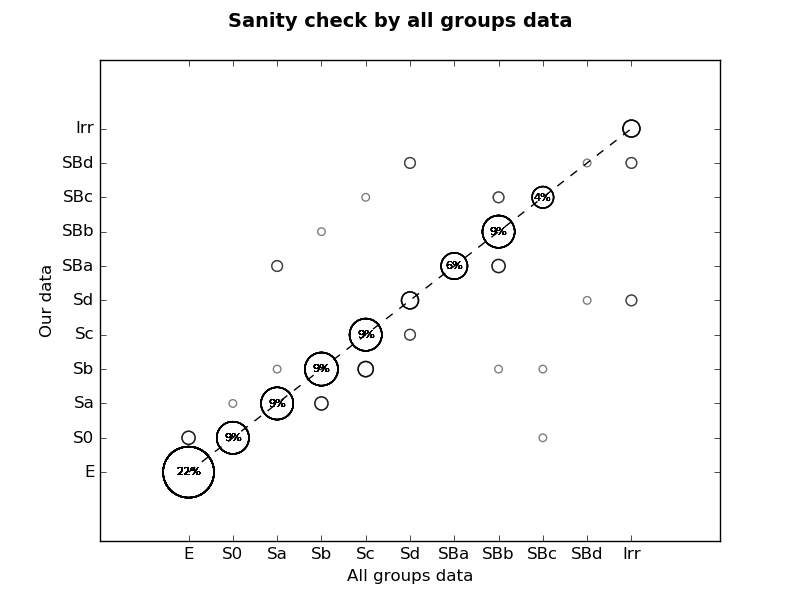
\includegraphics[width=6cm, height=4cm]{Sanity.png}
    \caption{Our data vs All groups }
   \end{figure}
   \column{.55\textwidth}
   \begin{figure}
    \centering
    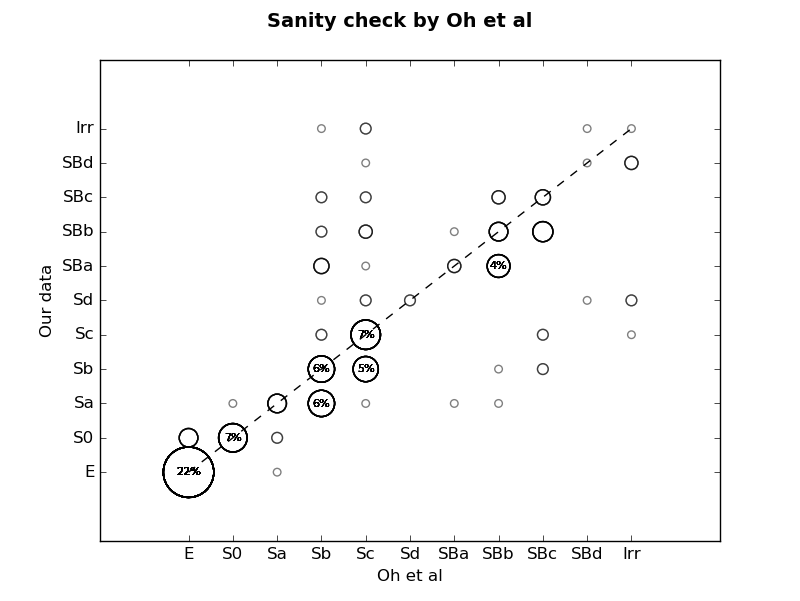
\includegraphics[width=6cm, height=4cm]{Sanity_oh.png}
    \caption{Our data vs Oh et al}
   \end{figure}
  \end{columns}

  \centering
 
\end{frame}

\begin{frame}
  \frametitle{Image Processing}
  
  - Feedback
  \begin{itemize}
   \item Morphology를 좀 더 정밀하게 분석하기 위해, Python의 OpenCV를 이용하여 다음과 같은 Image Processing을 하였다.
  \end{itemize}
  \begin{block}{Image Processing}
   \begin{enumerate}
   \item 주변의 극심한 Noise들을 제거하고 밝기를 평준화시키기 위하여 Tozero Thresholding을 이용하였다.
   \item Morphology를 좀더 쉽게 알아보기 위하여 Color convert로 image들을 Gray scale로 변경하였다.
   \item Figure의 dpi값을 조절하여 대비를 높였다.
   \end{enumerate}
  \end{block}

\end{frame}

\begin{frame}
 \frametitle{Image Processing}
 
 \begin{columns}[t]
  \column{.55\textwidth}
   \begin{figure}
    \centering
    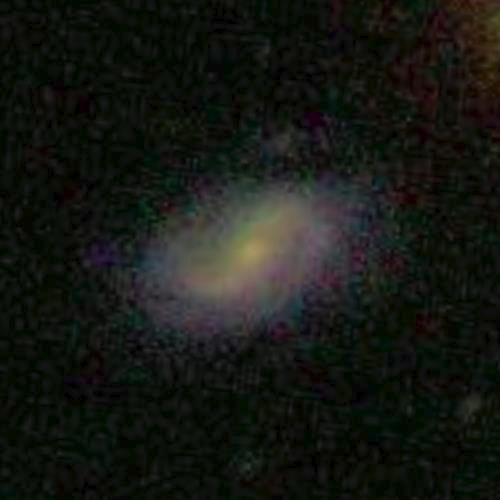
\includegraphics[width=6cm, height=4cm]{Test90.png}
    \caption{Original Image }
   \end{figure}
   \column{.55\textwidth}
   \begin{figure}
    \centering
    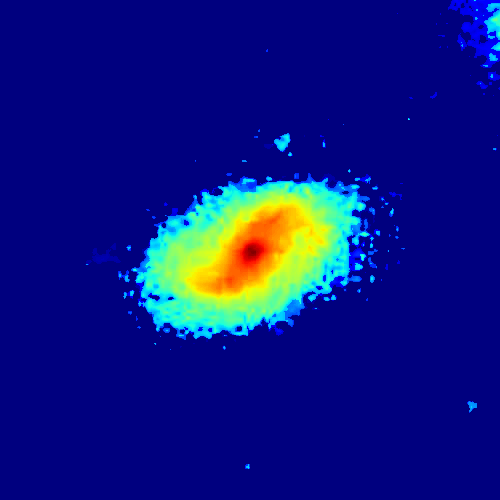
\includegraphics[width=6cm, height=4cm]{Conv90.png}
    \caption{Processed Image}
   \end{figure}
  \end{columns}

\end{frame}

\begin{frame}
  \frametitle{Image Processing}
  
  - Advantages
  \begin{itemize}
   \item Bulge의 크기가 아주 뚜렷하게 보인다.
   \item Bar의 여부를 판단하기 쉬우며 Arm의 Tightness가 아주 잘 관측된다.
   \item Bulge의 일그러짐이 잘 관측되어서 Irr의 분류가 쉬워졌다.
   \item 주변의 Noise들이 깔끔하게 사라져 Machine Learning 등의 용도로 사용하기 쉽다.
  \end{itemize}

\end{frame}

\begin{frame}
 \frametitle{Image Processing - Sanity Check}
 
 \begin{columns}[t]
  \column{.55\textwidth}
   \begin{figure}
    \centering
    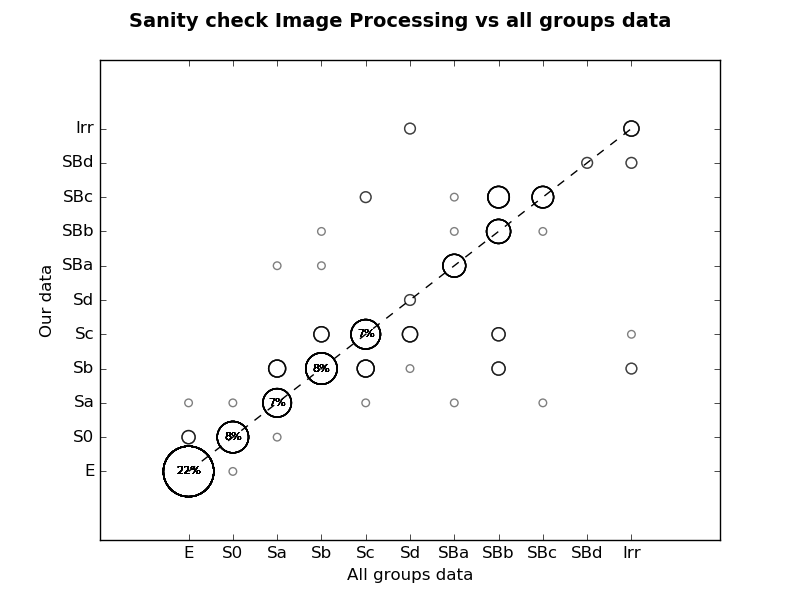
\includegraphics[width=6cm, height=4cm]{SanityIM_allgroup.png}
    \caption{Sanity Check by all groups}
   \end{figure}
   \column{.55\textwidth}
   \begin{figure}
    \centering
    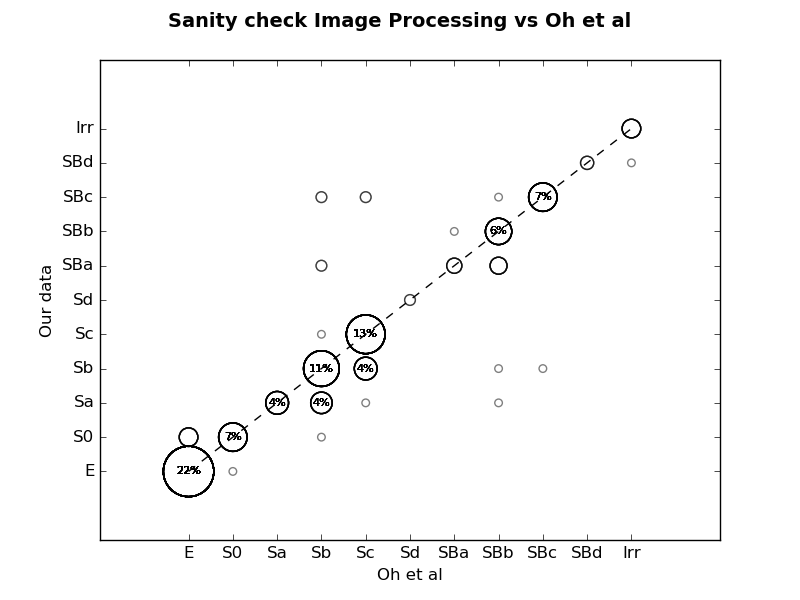
\includegraphics[width=6cm, height=4cm]{SanityIM_oh.png}
    \caption{Sanity Check by Oh et al}
   \end{figure}
  \end{columns}

\end{frame}

\begin{frame}
  \frametitle{Image Processing - Conclusion}
  \NM
  \begin{block}{Conclusion}
   \hspace{0.5cm}Group 평균 data와의 Matching accuracy는 감소한 반면, Oh et al과는 증가하였다는 점을 미루어 볼 때, Oh et al이 좀 더
   Trained eye에 가깝다는 것을 보여준다. \hspace{0.1cm}더불어 신뢰할만한 Oh et al 데이터와 상당히 흡사하다는 점을 볼 때,
   Morphology를 분류할 때에는 적절한 Image Processing은 필수 불가결하다는 것을 보여준다.
  \end{block}




\end{frame}
\endgroup

\section{Photometric Data}

\begin{frame}
  \frametitle{Introduction}
  \NM
  \begin{block}{Dataset}
  \begin{itemize}
   \item Photometric Data ; SDSS DR7
   \vspace{0.3cm}
   \item \textbf{Morphology : Oh et al. 2013}
  \end{itemize}
  \end{block}
  \vspace{0.3cm}
  \textbf{-What's New}
  \vspace{0.2cm}
  
\hspace{0.3cm}지난 과제에서는 단순히 SDSS DR7의 데이터에서 Morphology를 간접적으로 유추해내어 각 값들간의 관계를 살펴보았다면, 이번에는 Morphology 데이터를 따로
가져와 각 값간의 관계들을 살펴보았다.
 
\end{frame}

\begin{frame}
 \frametitle{FracdeV}
 \SM
 \begin{figure}
   \centering
    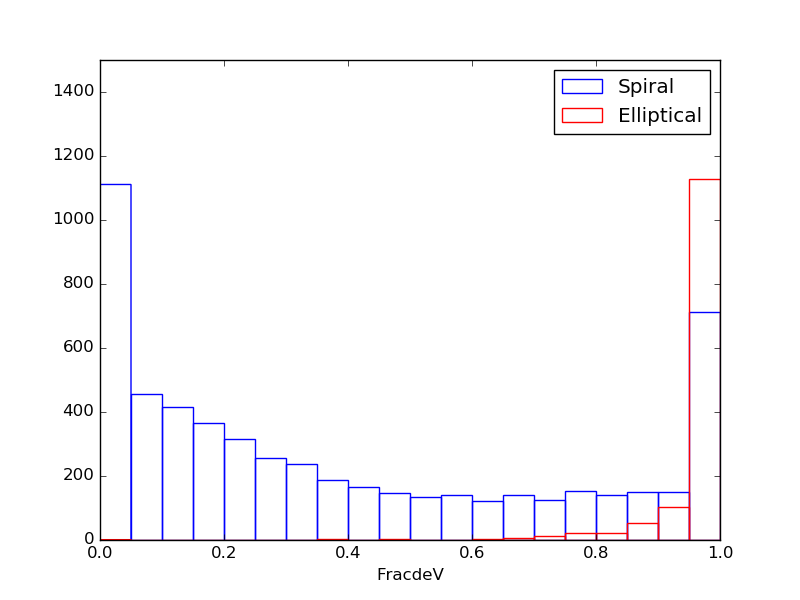
\includegraphics[width=8cm, height=5cm]{fracdev.png}
 \end{figure}

 \hspace{0.3cm}FracdeV의 경우, 1에 가까울 수록 Early Type에 가까움이 알려져 있기에 이를 \linebreak 확인해보았다. 그리고 우리가 사용한 데이터가 이와
일치하는 것을 확인할 수 있었지만, FracdeV가 1에 가까운 경우지만, 나선은하인 경우도 확인할 수 있었다.

 
\end{frame}

\begin{frame}
 \frametitle{Compactness}
 \SM
 \begin{columns}[t]
  \column{.55\textwidth}
   \begin{figure}
    \centering
    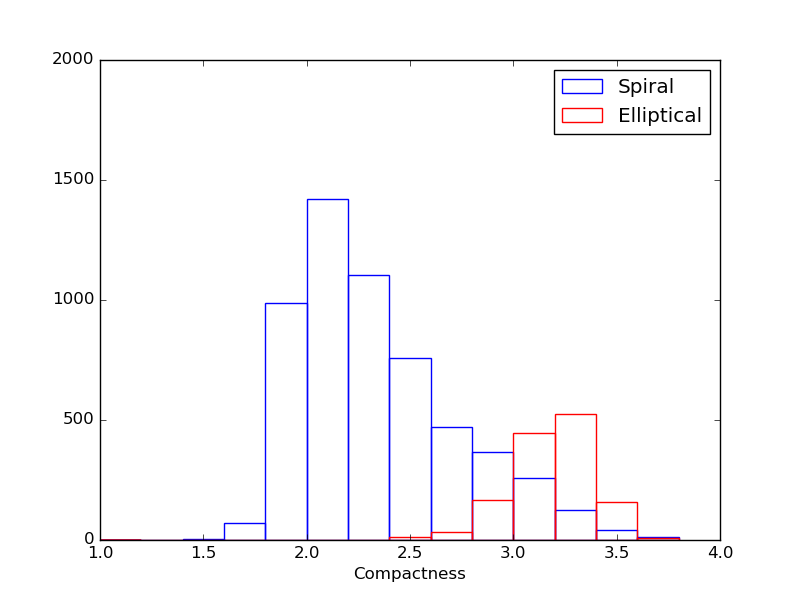
\includegraphics[width=6cm, height=4cm]{compact.png}
   \end{figure}
   \column{.55\textwidth}
   \begin{figure}
    \centering
    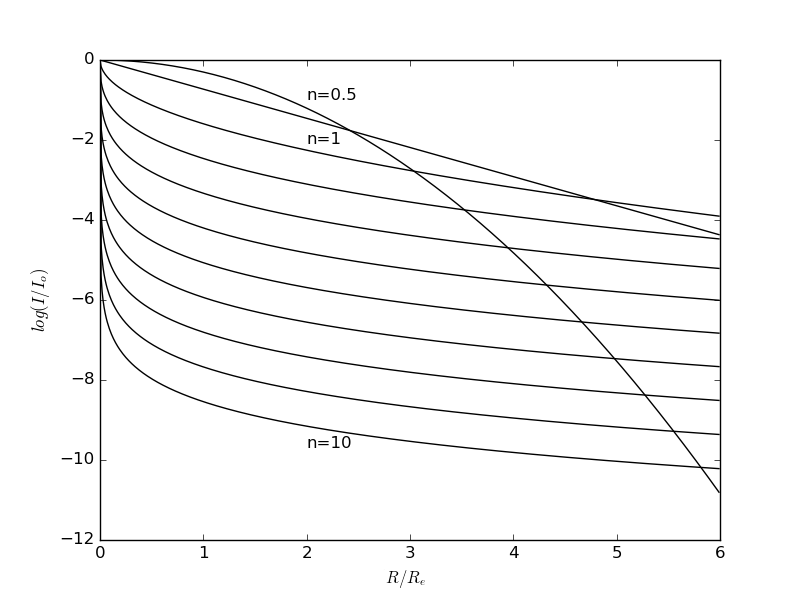
\includegraphics[width=6cm, height=4cm]{sersic.png}
   \end{figure}
  \end{columns}
\vspace{0.3cm}
Morphology에 따른 Compactness를 살펴보았을 때, 타원은하가 나선은하에 비해 더 Compact하다는 사실을 알 수 있다. 이는
은하의 Sersic Index와 Compactness간의 관계를 생각해보면 알 수 있다. Sersic Index가 높아질 수록 Compactness가 더 증
가할 것이라는 사실을 예상할 수 있다. 타원은하의 경우 Sersic Index가 나선은하에 비해 더 높으므로 자연스럽게 더 Compact하다
는 사실을 예상할 수 있다.

 
\end{frame}

\begin{frame}
 \frametitle{Ellipticity}
 \SM
 \begin{figure}
   \centering
    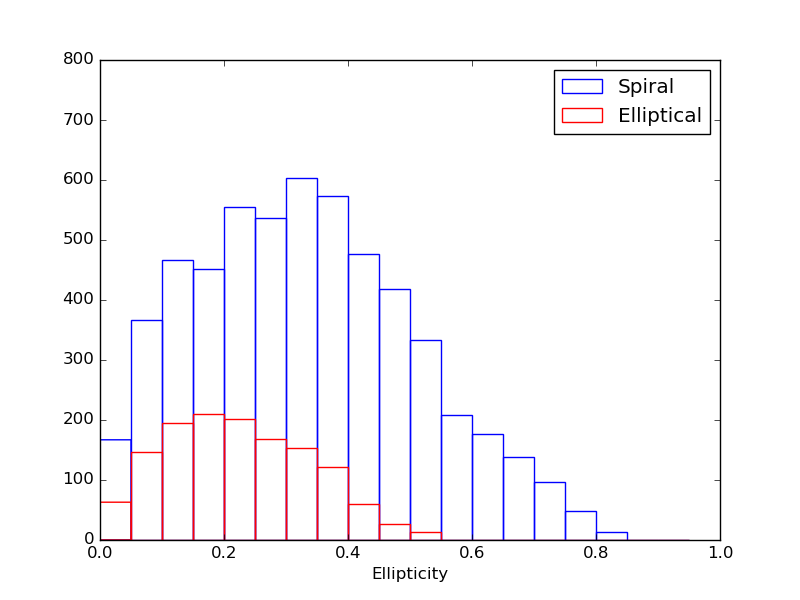
\includegraphics[width=8cm, height=5cm]{ellip.png}
 \end{figure}

Morphology에 따른 Ellipticity를 비교해보면 나선은하의 경우 Ellipticity의 범위가 타원은하에 비해 더 넓은 것을 확인할 수 있다.
이는 각 은하의 모양을 생각해보면 나선은하는 Disk를 가지므로 보이는 각도에 따라서 타원은하에 비해 Ellipticity가 증가할 수 있을
것이다.
 
\end{frame}

\begin{frame}
 \frametitle{Color-Magnitude Relation}
 \SSM
 \begin{columns}[t]
  \column{.55\textwidth}
   \begin{figure}
    \centering
    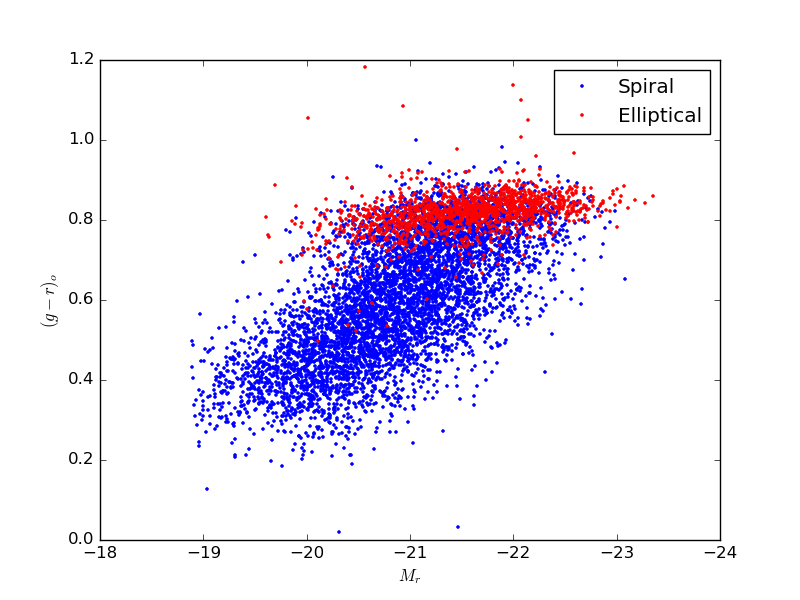
\includegraphics[width=6cm, height=4cm]{colormag.png}
   \end{figure}
   \column{.55\textwidth}
   \begin{figure}
    \centering
    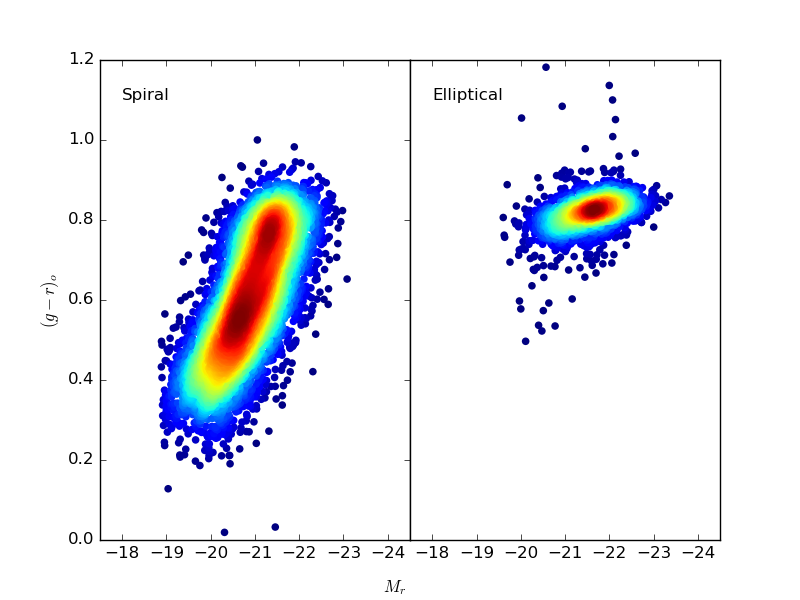
\includegraphics[width=6cm, height=4cm]{colormagdensity.png}
   \end{figure}
  \end{columns}
\vspace{0.3cm}
Color-Magnitude Diagram을 그린 결과, 우리가 잘 알고 있듯이 타원은하들에 대해선 Red Sequence를, 나선은하들에 대해선
Blue Cloud를 이루고 있음을 확인할 수 있었다. 나선 은하의 경우 Star Formation이 이뤄지고 있기에 대체적으로 color가 blue하
지만, 점차 시간에 지남에 따라 (이를 Magnitude가 점차 밝아지는 것으로 근사할 수 있다) gas를 다 소모하여 Star Formation이
점차 줄어들게 되어 color가 red해지는 변화를 확인할 수 있고, 타원 은하의 경우 Star Formation이 이미 매우 적어 모든 곳에서 대
체적으로 red하고 Magnitude가 밝아질 수록 더 red해지는 것을 확인할 수 있다.
이를 Contour로 확인해보면 Morphology에 따른 Color-Magnitude Diagram에서의 위치 차이를 더 자세하게 확인할 수 있다.
 
\end{frame}


\begin{frame}
 \frametitle{Size-Magnitude Relation}
 \SSM
 \begin{columns}[t]
  \column{.55\textwidth}
   \begin{figure}
    \centering
    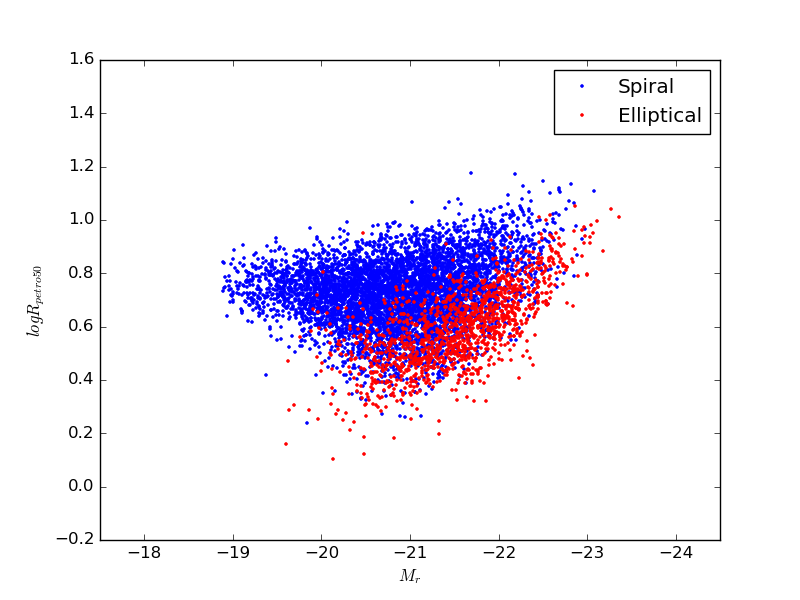
\includegraphics[width=6cm, height=4cm]{sizemag.png}
   \end{figure}
   \column{.55\textwidth}
   \begin{figure}
    \centering
    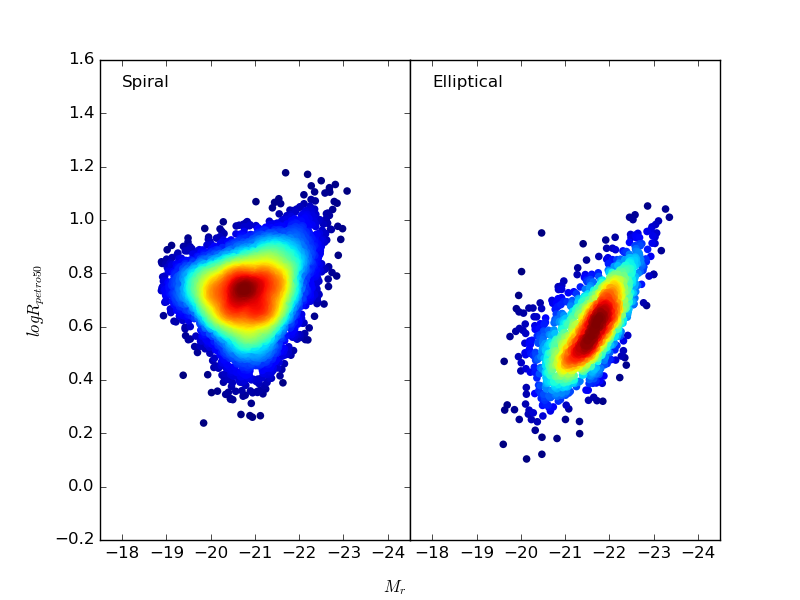
\includegraphics[width=6cm, height=4cm]{sizemagdensity.png}
   \end{figure}
  \end{columns}
\vspace{0.3cm}
앞에서 타원 은하가 나선은하에 비해 Magnitude가 더 밝은 것을 앞에서 확인할 수 있었다. 이를 바탕으로 Size – Magnitude간의
관계를 확인해보면, 타원은하에서 밝기가 증가할 수록 Half-Light Radius가 증가하는 것을 확인할 수 있었다. 이는 잎에서 Magni-
tude를 대략적으로 만들어진 별의 개수로 생각한다면 자연스럽게 Magnitude가 밝아질 수록, Size가 증가할 것으로 예상할 수 있다.
하지만 나선은하의 경우 타원은하와 달리 단순한 증가-감소 추세를 보이지는 않는데, 나선은하는 은하마다 Star Formation의 정도
차이가 크므로 단순한 Sequence로 나타나지 않음을 예상할 수 있다.

 
\end{frame}


\begin{frame}
 \frametitle{Size-Mass Relation}
 \SSM
 \begin{columns}[t]
  \column{.55\textwidth}
   \begin{figure}
    \centering
    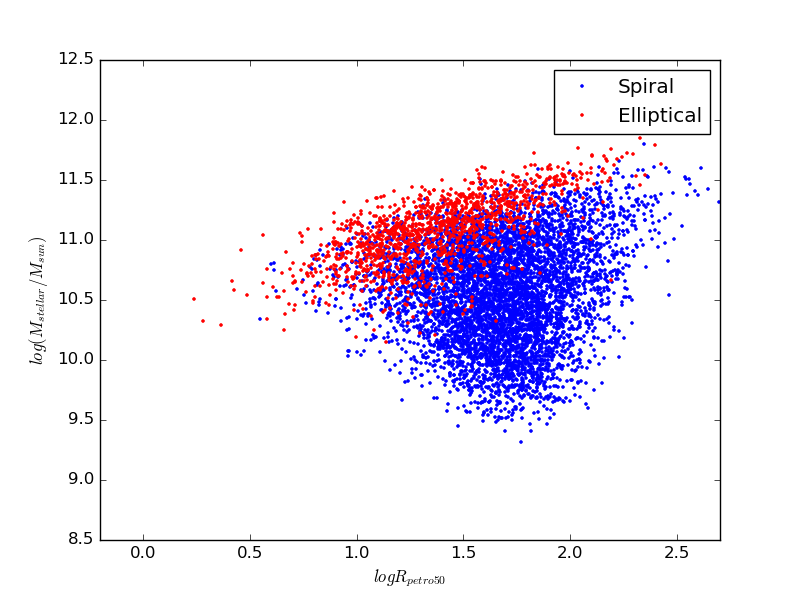
\includegraphics[width=6cm, height=4cm]{sizemass.png}
   \end{figure}
   \column{.55\textwidth}
   \begin{figure}
    \centering
    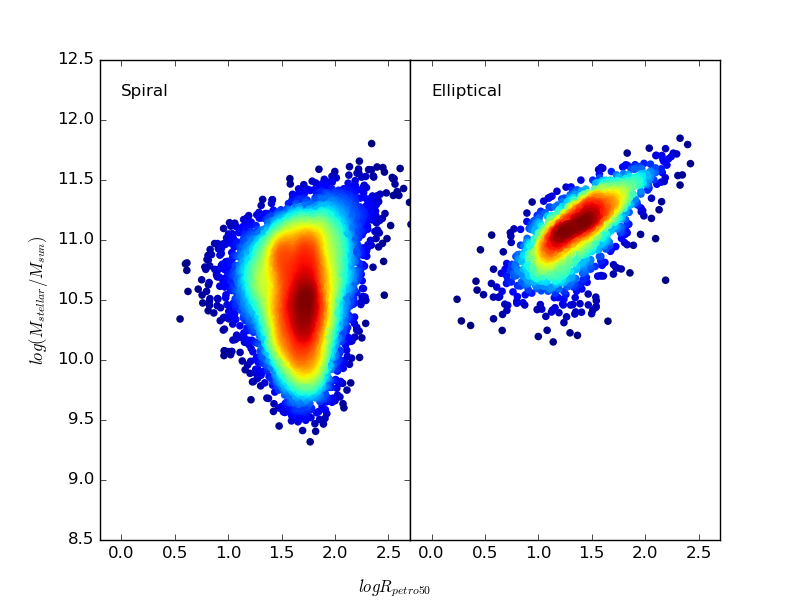
\includegraphics[width=6cm, height=4cm]{sizemassdensity.png}
   \end{figure}
  \end{columns}
\vspace{0.3cm}
Morphology에 따른 Size – Mass Relation을 확인해보면 앞에서의 Size – Magnitude Relation과 비슷한 양상을 확인할 수 있
다. 타원은하에선 Stellar Mass가 증가할 수록 Size가 같이 증가하는 것을 확인할 수 있고, 나선은하에선 은하간의 차이가 심하기에
단순한 증가 추세로 나타나지 않는 것을 확인할 수 있었다.

\end{frame}

\begin{frame}
 \frametitle{Mass-Mean Surface Brightness Relation}
 \SSM
 \begin{columns}[t]
  \column{.55\textwidth}
   \begin{figure}
    \centering
    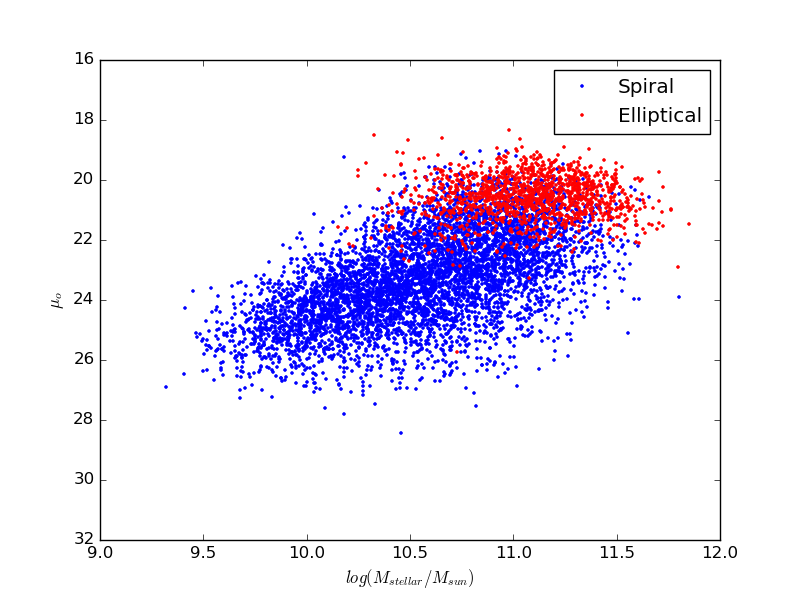
\includegraphics[width=6cm, height=4cm]{masssurf.png}
   \end{figure}
   \column{.55\textwidth}
   \begin{figure}
    \centering
    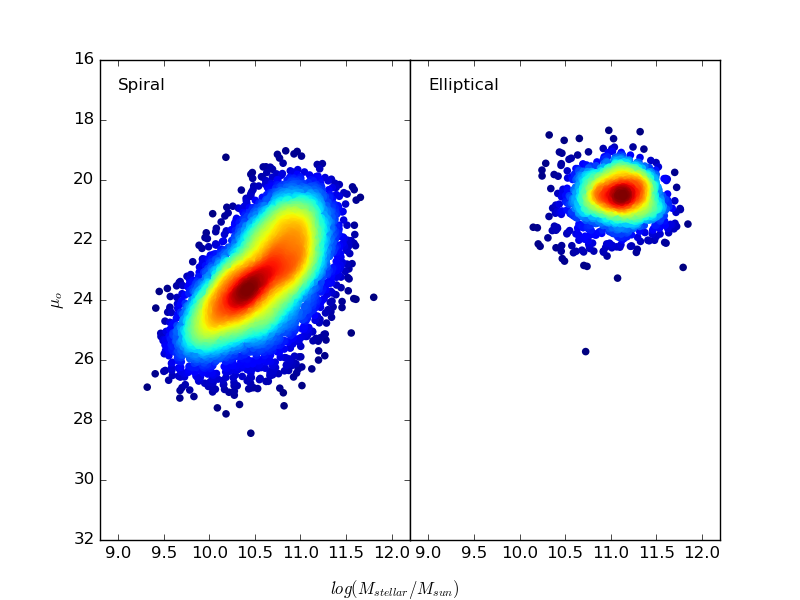
\includegraphics[width=6cm, height=4cm]{masssurfdensity.png}
   \end{figure}
  \end{columns}
\vspace{0.3cm}
우선 나선 은하의 경우 다양한 Stellar Mass를 가지는 것을 확인할 수 있고, 타원 은하의 경우 많은 Merging을 겪어서 나선 은하에
비해 Stellar Mass가 더 큰 것을 확인할 수 있다. 이에 더 나아가 Mean Surface Brightness와의 관계를 살펴보면, 나선 은하에서
Stellar Mass가 증가할 수록, Mean Surface Brightness가 증가하는 것을 확인할 수 있다. 나선은하가 Star Formation이 일어
나는 중인 은하이므로 별이 많이 만들어질 수록 그 밝기와 Stellar Mass가 같이 증가할 것임을 알 수 있고, 타원 은하의 경우에는
Star Formation이 거의 일어나지 않기 때문에, Stellar Mass가 증가하더라도 밝기의 변화가 거의 없는 것으로 볼 수 있을 것이다.
\end{frame}

\begin{frame}
 \frametitle{Barred Spiral Galaxy vs Normal Spiral Galaxy}
 \SSM
 \begin{columns}[t]
  \column{.55\textwidth}
   \begin{figure}
    \centering
    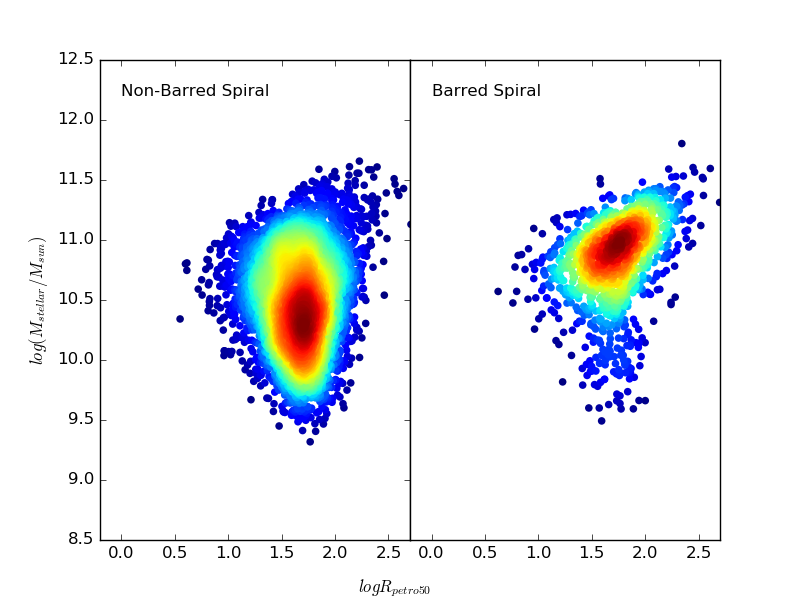
\includegraphics[width=6cm, height=4cm]{sizemassdensity2.png}
   \end{figure}
   \column{.55\textwidth}
   \begin{figure}
    \centering
    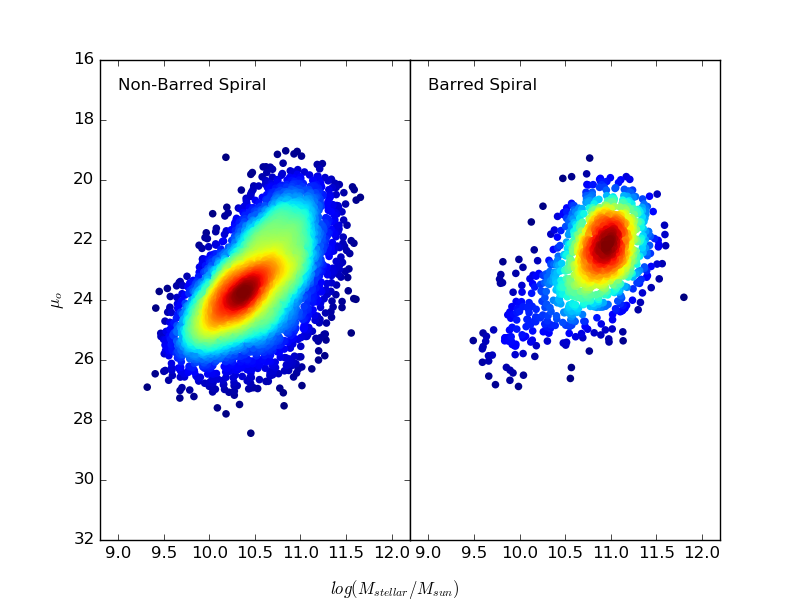
\includegraphics[width=6cm, height=4cm]{masssurfdensity2.png}
   \end{figure}
  \end{columns}
\vspace{0.3cm}
우선 나선 은하의 경우 다양한 Stellar Mass를 가지는 것을 확인할 수 있고, 타원 은하의 경우 많은 Merging을 겪어서 나선 은하에
비해 Stellar Mass가 더 큰 것을 확인할 수 있다. 이에 더 나아가 Mean Surface Brightness와의 관계를 살펴보면, 나선 은하에서
Stellar Mass가 증가할 수록, Mean Surface Brightness가 증가하는 것을 확인할 수 있다. 나선은하가 Star Formation이 일어
나는 중인 은하이므로 별이 많이 만들어질 수록 그 밝기와 Stellar Mass가 같이 증가할 것임을 알 수 있고, 타원 은하의 경우에는
Star Formation이 거의 일어나지 않기 때문에, Stellar Mass가 증가하더라도 밝기의 변화가 거의 없는 것으로 볼 수 있을 것이다.
\end{frame}

\begin{frame}
 \frametitle{Barred Spiral Galaxy vs Normal Spiral Galaxy}
 \SSM
 \begin{columns}[t]
  \column{.55\textwidth}
   \begin{figure}
    \centering
    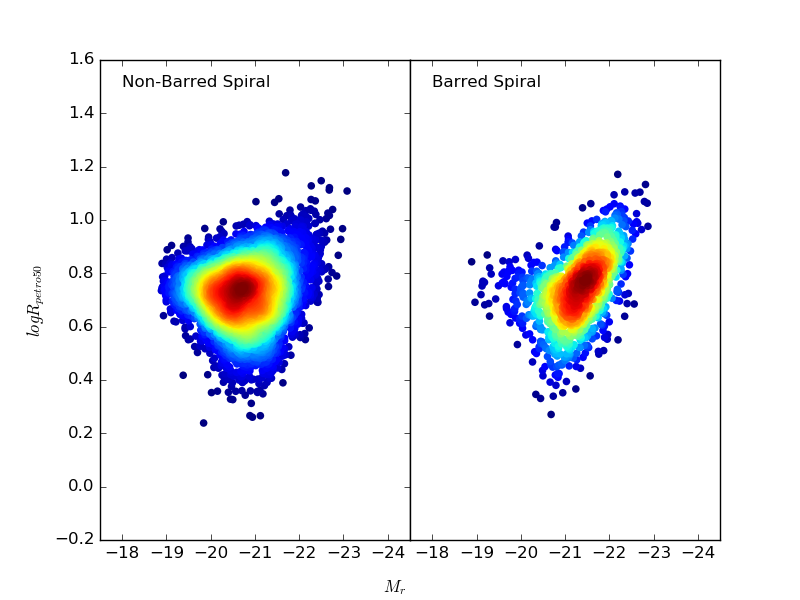
\includegraphics[width=6cm, height=4cm]{sizemagdensity2.png}
   \end{figure}
   \column{.55\textwidth}
   \begin{figure}
    \centering
    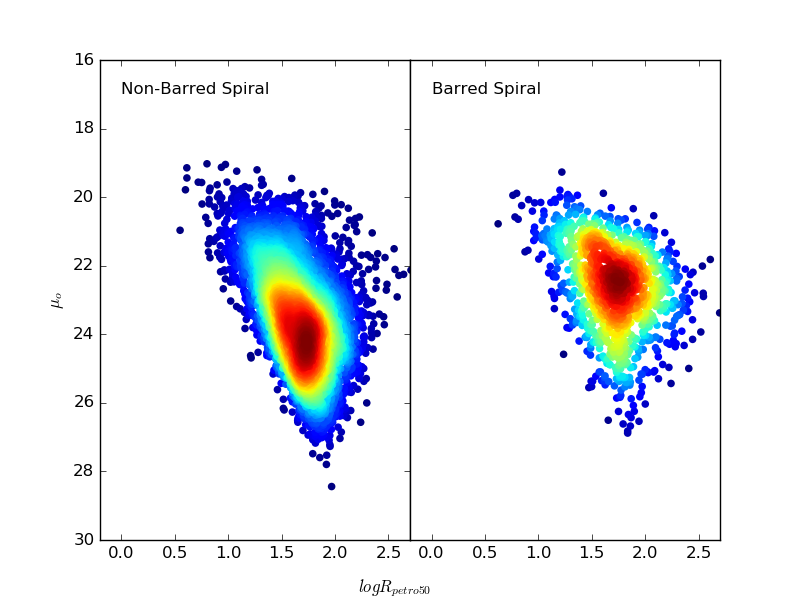
\includegraphics[width=6cm, height=4cm]{sizesurfdensity2.png}
   \end{figure}
  \end{columns}
\vspace{0.3cm}
우선 나선 은하의 경우 다양한 Stellar Mass를 가지는 것을 확인할 수 있고, 타원 은하의 경우 많은 Merging을 겪어서 나선 은하에
비해 Stellar Mass가 더 큰 것을 확인할 수 있다. 이에 더 나아가 Mean Surface Brightness와의 관계를 살펴보면, 나선 은하에서
Stellar Mass가 증가할 수록, Mean Surface Brightness가 증가하는 것을 확인할 수 있다. 나선은하가 Star Formation이 일어
나는 중인 은하이므로 별이 많이 만들어질 수록 그 밝기와 Stellar Mass가 같이 증가할 것임을 알 수 있고, 타원 은하의 경우에는
Star Formation이 거의 일어나지 않기 때문에, Stellar Mass가 증가하더라도 밝기의 변화가 거의 없는 것으로 볼 수 있을 것이다.
\end{frame}

\begin{frame}
 \frametitle{Barred Spiral Galaxy vs Normal Spiral Galaxy}
 \SSM
 \begin{columns}[t]
  \column{.55\textwidth}
   \begin{figure}
    \centering
    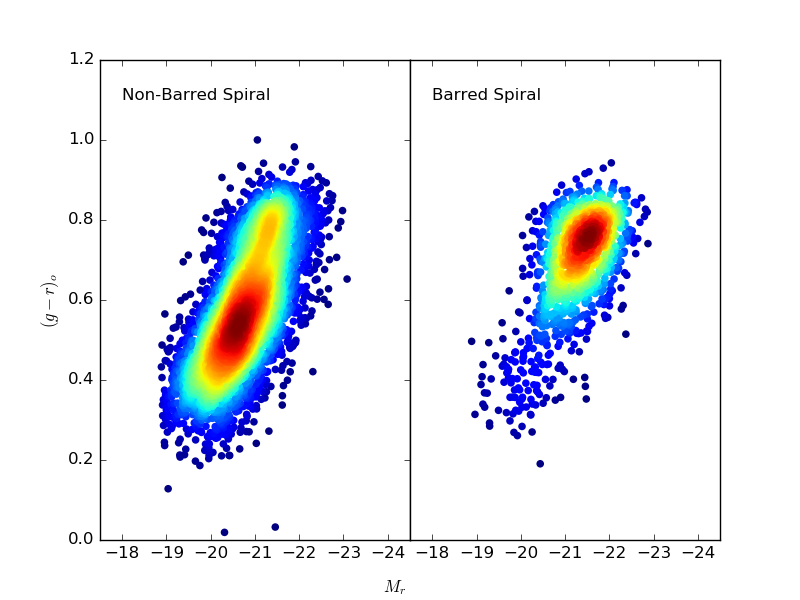
\includegraphics[width=6cm, height=4cm]{colormagdensity2.png}
   \end{figure}
   \column{.55\textwidth}
   \begin{figure}
    \centering
    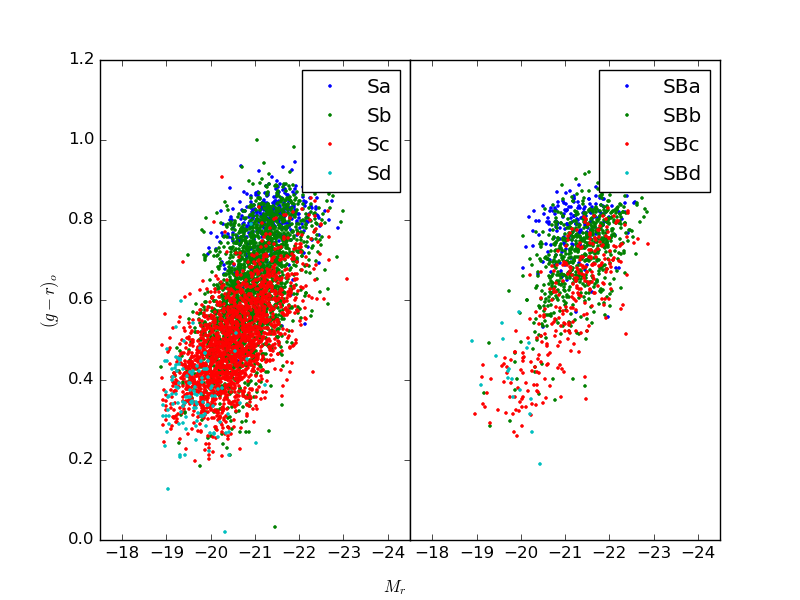
\includegraphics[width=6cm, height=4cm]{what.png}
   \end{figure}
  \end{columns}
\vspace{0.3cm}
우선 나선 은하의 경우 다양한 Stellar Mass를 가지는 것을 확인할 수 있고, 타원 은하의 경우 많은 Merging을 겪어서 나선 은하에
비해 Stellar Mass가 더 큰 것을 확인할 수 있다. 이에 더 나아가 Mean Surface Brightness와의 관계를 살펴보면, 나선 은하에서
Stellar Mass가 증가할 수록, Mean Surface Brightness가 증가하는 것을 확인할 수 있다. 나선은하가 Star Formation이 일어
나는 중인 은하이므로 별이 많이 만들어질 수록 그 밝기와 Stellar Mass가 같이 증가할 것임을 알 수 있고, 타원 은하의 경우에는
Star Formation이 거의 일어나지 않기 때문에, Stellar Mass가 증가하더라도 밝기의 변화가 거의 없는 것으로 볼 수 있을 것이다.
\end{frame}

\section{Absorption Line Properties}

\begin{frame}
  \frametitle{Introduction}
  \NM
  \begin{block}{Dataset}
  \begin{itemize}
   \item Photometric Data ; SDSS DR7
   \vspace{0.3cm}
   \item Spectroscopic Data : OSSY Database
   \vspace{0.3cm}
   \item Morphology : Oh et al. 2013
  \end{itemize}
  \end{block}
  \vspace{0.3cm}
  \textbf{-Introduction}
  \vspace{0.2cm}
  
\hspace{0.3cm}HW4에서는 Morphology에 따른 Absorption Line의 특징을 확인하고,
Spectroscopic Data와 Photometric Data와의 관계를 확인해보았다.
\end{frame}

\begin{frame}
 \frametitle{Color-Velocity Dispersion}
 \SSM
 \begin{figure}
    \centering
    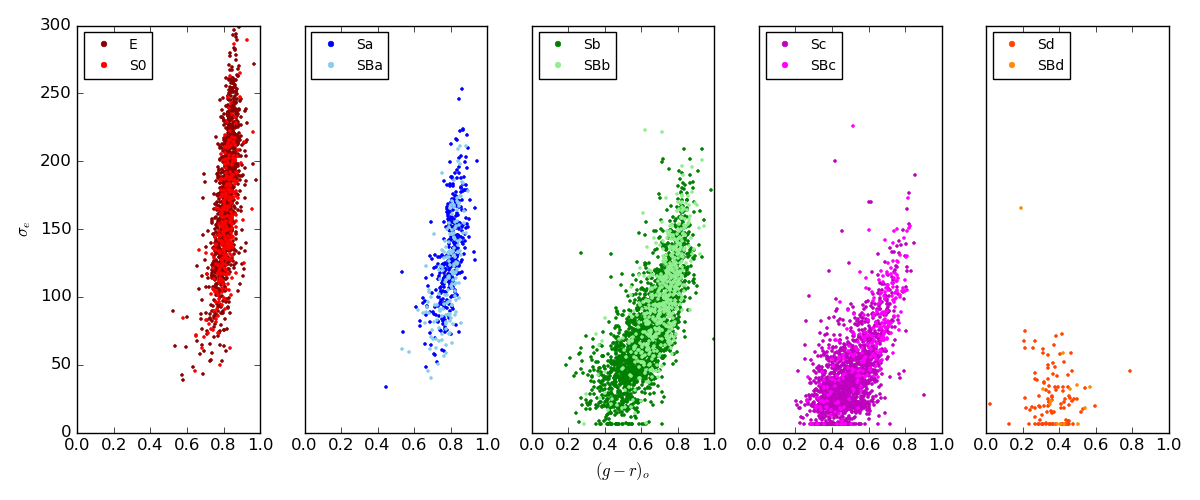
\includegraphics[width=8cm, height=5cm]{colorsigma.png}
 \end{figure}
\vspace{0.2cm}
Color에 따른 Velocity Dispersion을 확인하면 color가 red해질수록 velocity dispersion이 증가하는 것을 확인할 수 있다. 이
에 더 나아가 Morphology의 변화에 따른 Color-Velocity Dispersion Relation을 확인해보았다. 이를 통해 Late-Type으로 갈수
록 color가 blue해질수록 dispersion이 같이 감소하는 형태를 확인할 수 있었다.
\end{frame}

\begin{frame}
 \frametitle{Mass-Velocity Dispersion}
 \SSM
 \begin{figure}
    \centering
    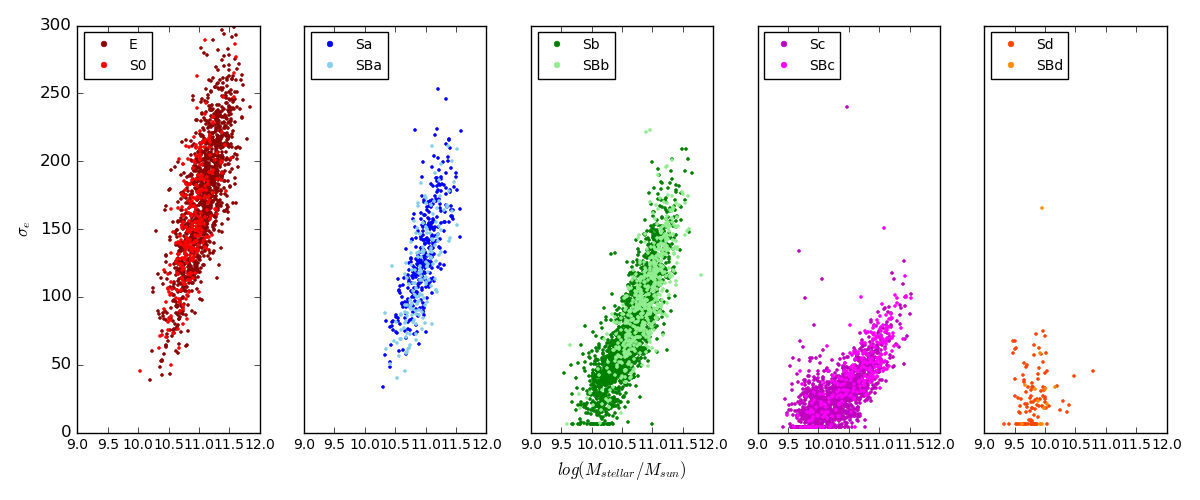
\includegraphics[width=8cm, height=5cm]{masssigma.png}
 \end{figure}
\vspace{0.2cm}
Color와 Stellar Mass간의 양의 상관관계가 존재하는 만큼 Mass-Velocity Dispersion Diagram은 Color-Velocity Disper-
sion Diagram과 비슷한 형태를 취할 것이라는 것을 예상할 수 있었고, 실제 확인한 결과 예상과 맞아 떨어졌다. Late Type으로 갈
수록 Stellar Mass가 감소하고 Velocity Dispersion도 같이 감소하는 형태를 확인할 수 있었다.
Stellar Mass가 증가할 수록 Velocity Dispersion이 증가하는 형태에 대해선 Virial Theorem에 의해 가 성립하므로 나타나는 것
으로 예측할 수 있다.
\end{frame}

\begin{frame}
 \frametitle{Type-Velocity Dispersion}
 \SSM
  \begin{columns}[t]
  \column{.55\textwidth}
   \begin{figure}
    \centering
    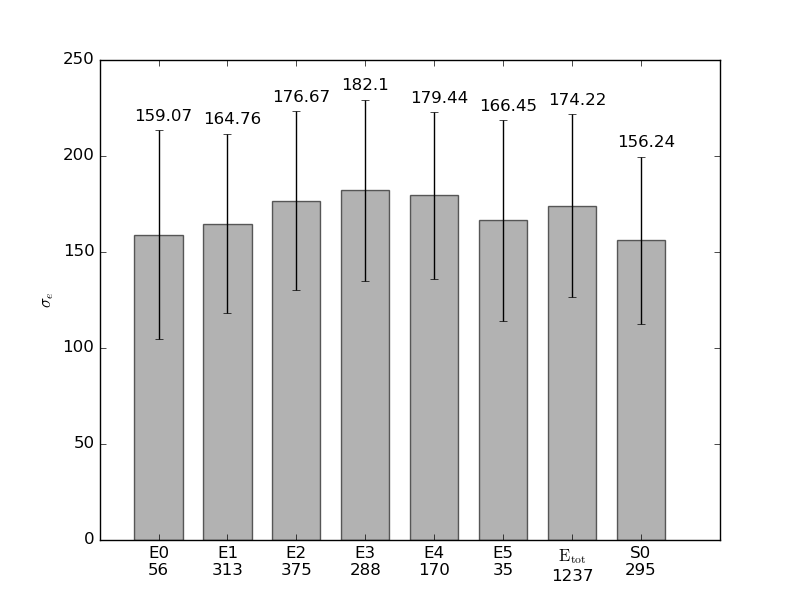
\includegraphics[width=6cm, height=4cm]{elsigma.png}
   \end{figure}
   \column{.55\textwidth}
   \begin{figure}
    \centering
    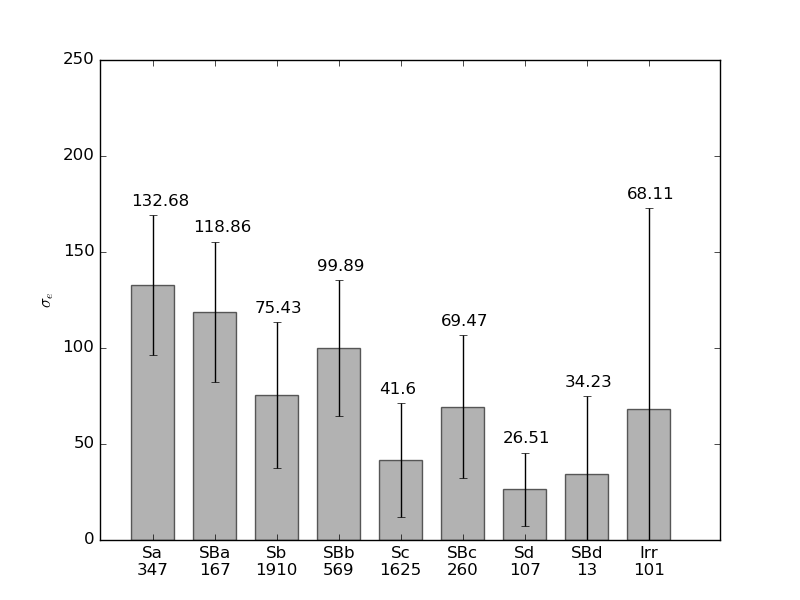
\includegraphics[width=6cm, height=4cm]{spsigma.png}
   \end{figure}
  \end{columns}
\vspace{0.2cm}
Morphological Type에 따른 Velocity Dispersion을 살펴볼 경우, 타원은하에 대해선 주목할만한 차이가 존재하지 않는다. 이는
앞의 HW3에서 확인했던 것을 통해 충분히 예측할 수 있다.
하지만 나선은하의 경우 Late Type으로 갈 수록 Velocity Dispersion이 감소하는 경향성을 보여주는데, 이는 앞에서 확인했듯이
Late Type으로 갈수록 Stellar Mass가 감소하고 Virial Theorem에 의해 Velocity Dispersion도 같이 낮아짐을 알 수 있다.
불규칙은하에서는 Merging등의 다양한 활동이 일어나는 은하이기에 Velocity Dispersion 값이 매우 다양하게 측정되는 것(Error
Bar를 통해)을 확인할 수 있었다.
\end{frame}

\begin{frame}
 \frametitle{Type-H$\beta$}
 \SSM
  \begin{columns}[t]
  \column{.55\textwidth}
   \begin{figure}
    \centering
    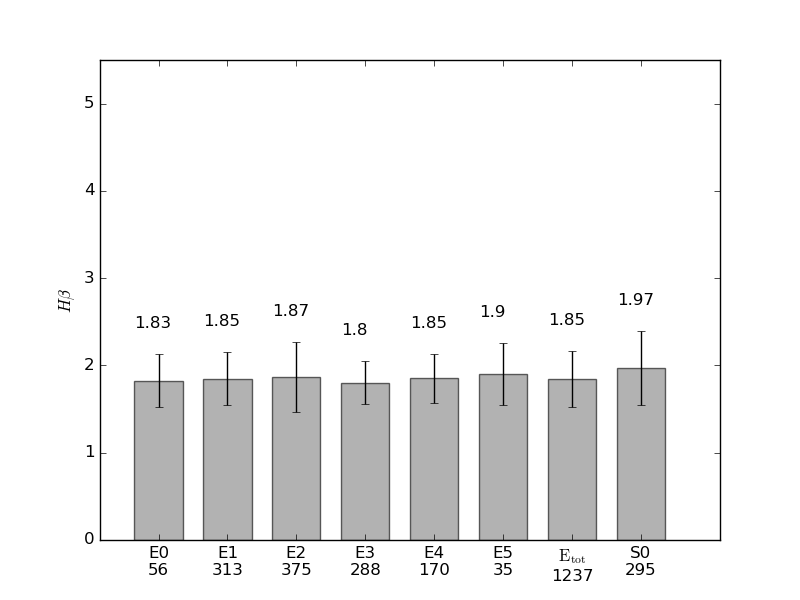
\includegraphics[width=6cm, height=4cm]{elhb.png}
   \end{figure}
   \column{.55\textwidth}
   \begin{figure}
    \centering
    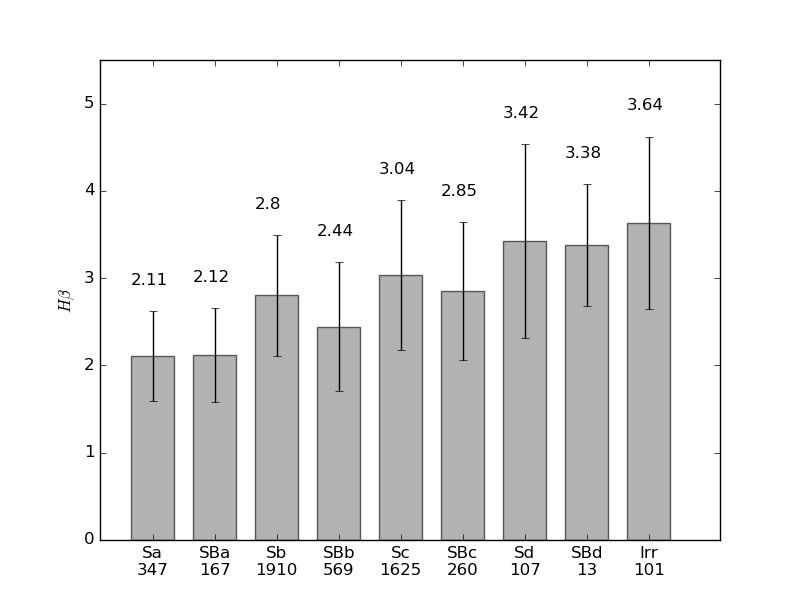
\includegraphics[width=6cm, height=4cm]{sphb.png}
   \end{figure}
  \end{columns}
\vspace{0.2cm}
H$\beta$은 대략 10000K에서 가장 강하게 나타나는 흡수선으로써, old한 stellar population에선 잘 나타나지 않는 특성을 가지고 있
다. (Khim et al. 2015) 이를 통해 위의 그림을 살펴보면, 타원은하에서는 모두 다 비슷한 값을 나타내지만 나선은하와 비교해서 적
은 값을 가지는 것을 확인할 수 있고, 나선은하 내에선 Late Type으로 갈 수록 흡수선의 세기가 증가하는 것을 볼 수 있다는 점이다.
거기에서 더 나아가, 불규칙 은하에서 가장 세기가 크게 나타나는데, 앞에서 Velocity Dispersion의 값이 불규칙 은하에선 매우 다양
하게 나타났던 것과 비교하면 상대적으로 일관적인 값으로 보인다. 이를 통해 주로 불규칙은하를 만드는 Merging등의 활동이 Star
Formation을 촉진시킨다는 점을 예측할 수도 있다.
\end{frame}

\begin{frame}
 \frametitle{Type-Fe5270}
 \SSM
  \begin{columns}[t]
  \column{.55\textwidth}
   \begin{figure}
    \centering
    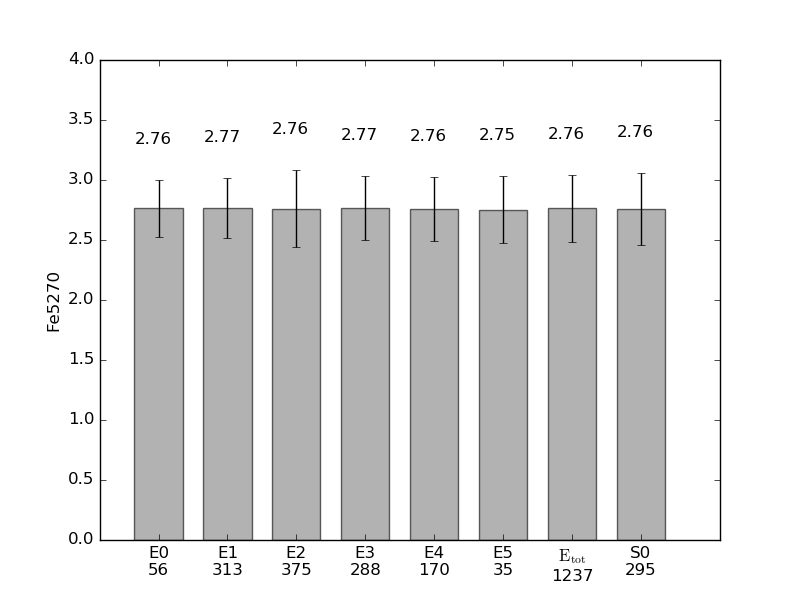
\includegraphics[width=6cm, height=4cm]{elfe.png}
   \end{figure}
   \column{.55\textwidth}
   \begin{figure}
    \centering
    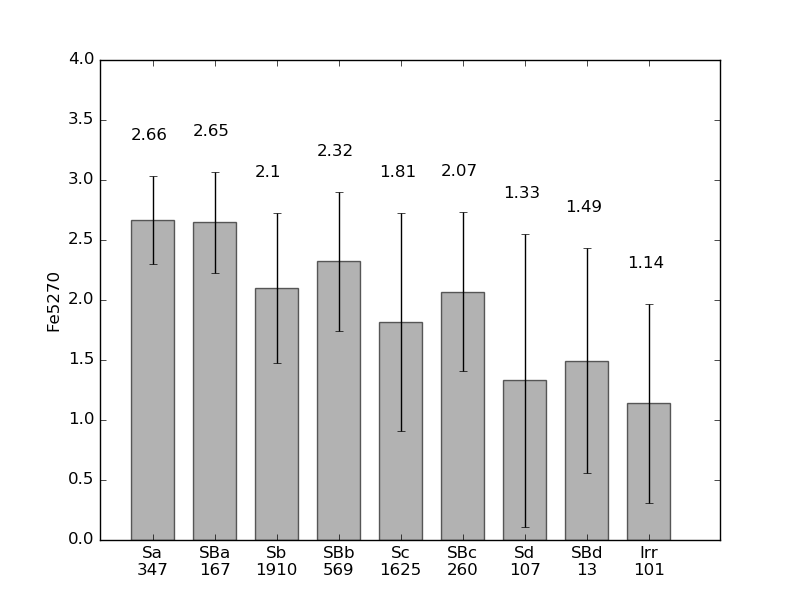
\includegraphics[width=6cm, height=4cm]{spfe.png}
   \end{figure}
  \end{columns}
\vspace{0.2cm}
Fe5270은 은하의 Metallcitiy에 대한 좋은 지표 중 하나이다. 이를 통해 위의 그림을 살펴보면 타원은하는 나선은하에 비해 Metal-
rich하다는 사실을 알 수 있고, 나선은하의 경우 Late Type으로 갈수록 Metal-Poor하다는 사실을 알 수 있다. 또한 불규칙 은하의
경우 다른 Morphological Type에 비해 제일 흡수선의 세기가 약하다는 사실을 통해 앞의 Type – H$\beta$ 에서 얻은 결론을 똑같이 적용
할 수 있을 것으로 예상된다.
\end{frame}

\begin{frame}
 \frametitle{Type-Mgb}
 \SSM
  \begin{columns}[t]
  \column{.55\textwidth}
   \begin{figure}
    \centering
    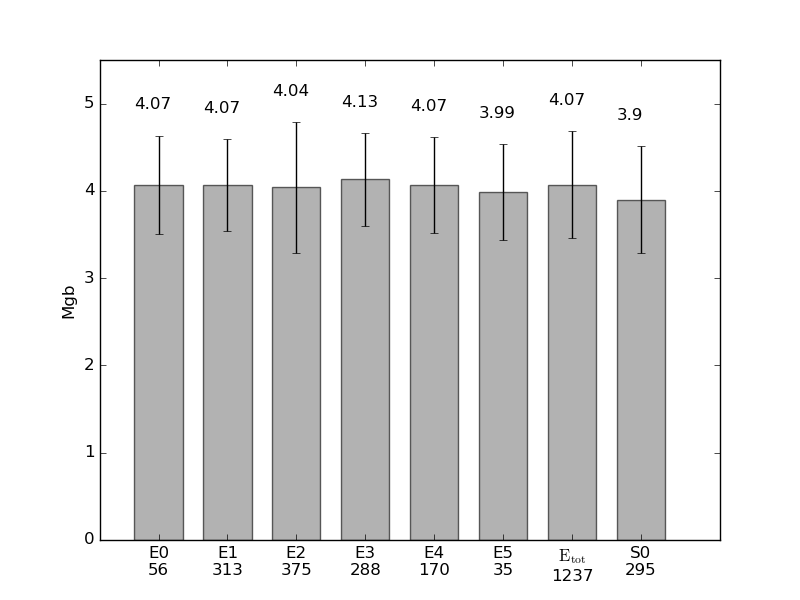
\includegraphics[width=6cm, height=4cm]{elmg.png}
   \end{figure}
   \column{.55\textwidth}
   \begin{figure}
    \centering
    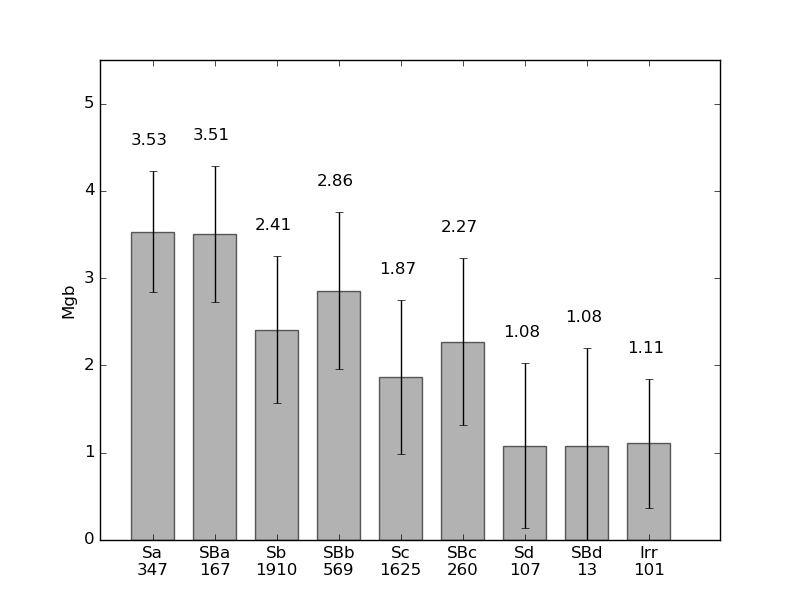
\includegraphics[width=6cm, height=4cm]{spmg.png}
   \end{figure}
  \end{columns}
\vspace{0.2cm}
Mgb 흡수선은 Metallicity의 지표가 되기도 하지만, $\alpha$-element의 지표가 되는 흡수선이다. $\alpha$-element는 Supernovae Type II
을 통해 주로 형성되는데, 위의 그림을 통해 나선은하에 비해 타원은하에 상대적으로 $\alpha$-element의 양이 많을 것이라고 예상할 수 있
고, 또한 나선은하 내에선 Late Type으로 갈수록 $\alpha$-element의 양이 감소하는 것을 확인할 수 있다.
\end{frame}

\begin{frame}
 \frametitle{Type-Mgb}
 \SSM
  \begin{columns}[t]
  \column{.55\textwidth}
   \begin{figure}
    \centering
    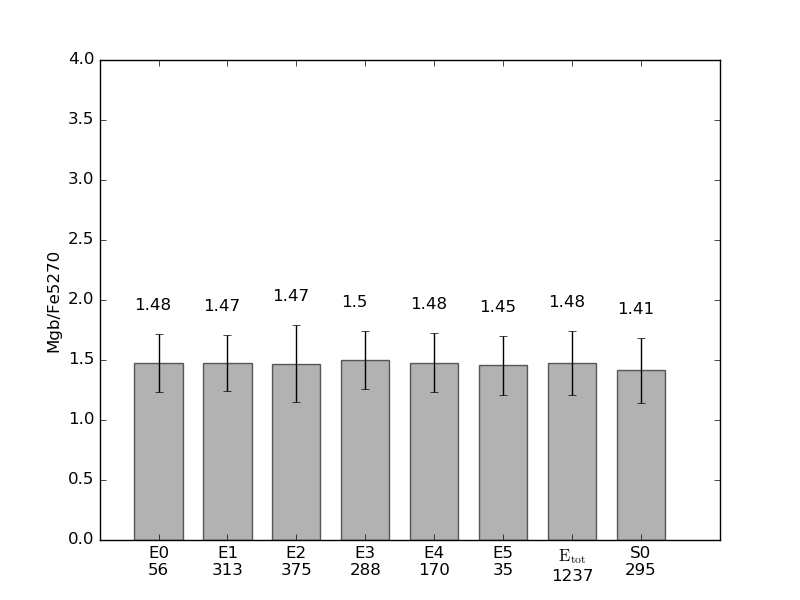
\includegraphics[width=6cm, height=4cm]{elmg2.png}
   \end{figure}
   \column{.55\textwidth}
   \begin{figure}
    \centering
    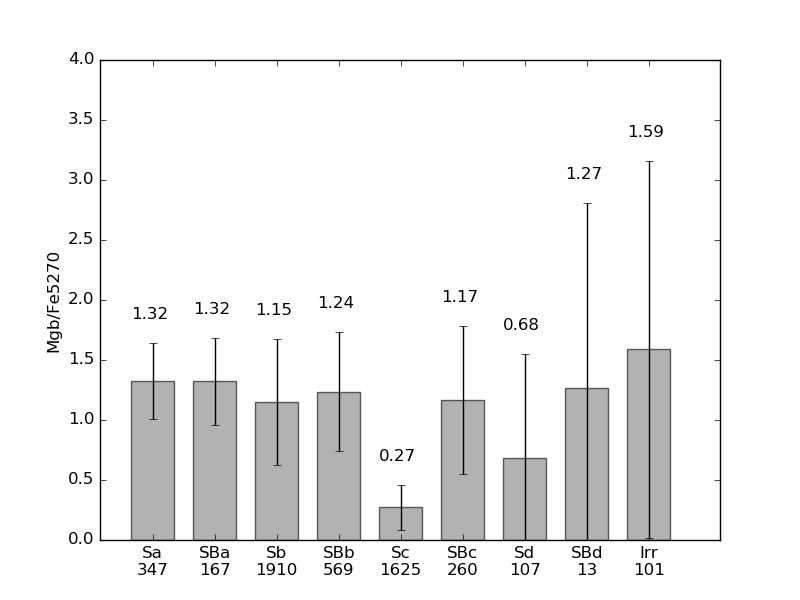
\includegraphics[width=6cm, height=4cm]{spmg2.png}
   \end{figure}
  \end{columns}
\vspace{0.2cm}
Mgb 흡수선은 Metallicity의 지표가 되기도 하지만, $\alpha$-element의 지표가 되는 흡수선이다. $\alpha$-element는 Supernovae Type II
을 통해 주로 형성되는데, 위의 그림을 통해 나선은하에 비해 타원은하에 상대적으로 $\alpha$-element의 양이 많을 것이라고 예상할 수 있
고, 또한 나선은하 내에선 Late Type으로 갈수록 $\alpha$-element의 양이 감소하는 것을 확인할 수 있다.
\end{frame}

\begin{frame}
 \frametitle{Fundamental Plane}
 \SSM
   \begin{figure}
    \centering
    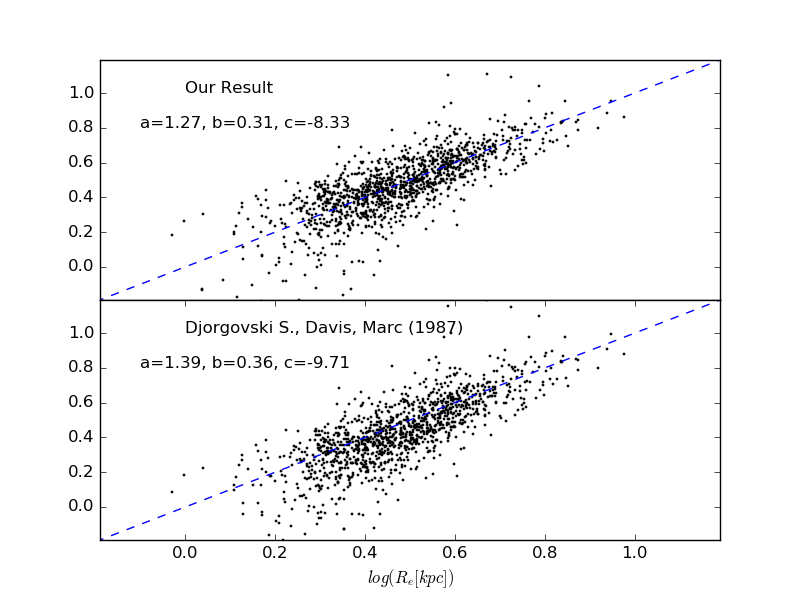
\includegraphics[width=7cm, height=5cm]{fundplane1.png}
   \end{figure}

\vspace{0.2cm}
타원은하에 있어서 주요한 Scaling Relation으로 타원은하의 크기, 속도 분산, 밝기 간의 Fundamental Plane이 존재한다. 우리
가 가진 데이터를 통해 Fundamental Plane을 구하고 이를 알려진 값들과 비교해보았다. 지난 과제에서는 여러 어려움 때문에 문헌
을 참고하여 b값(Hoessel, J. G.,Schneider, D. P. 1985)을 고정시킨 뒤, a를 Least Square Fitting을 통해 구하였다. 이번에는
다른 방식으로 a값을 변화를 줘가면서 Least Square Fitting을 통해 가장 낮은 을 주는 a,b,c값을 찾았고 그 것이 바로 위의 결과이다.
\end{frame}

\section{Emission Line Properties}

\begin{frame}
  \frametitle{BPT Diagram}
  \SM
  \begin{figure}
    \centering
    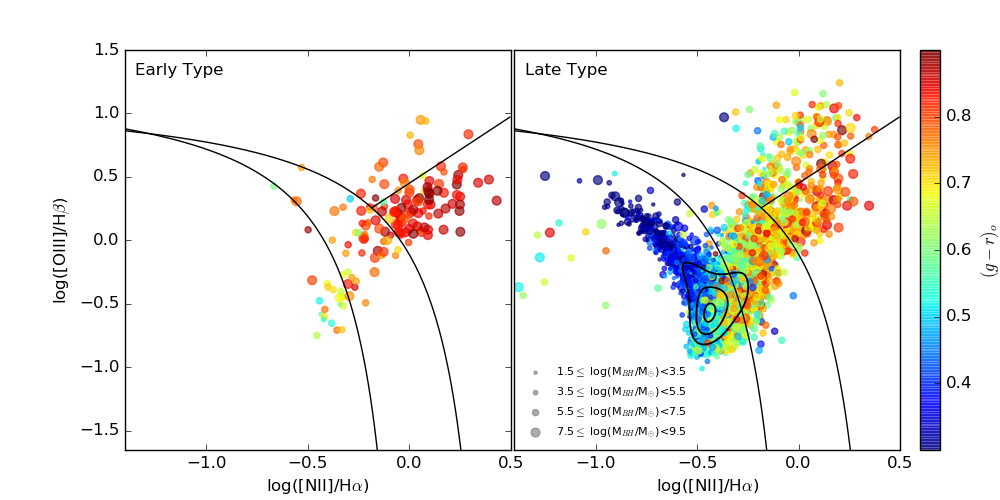
\includegraphics[width=10cm, height=4.5cm]{BPT.png}
   \end{figure}
  \vspace{0.2cm}

  \begin{itemize}
   \item Early type galaxy들은 LINER 계열에 많이 분포하고 있고, Late type galaxy들은 Star forming 계열에 많이 분포하고 있음.
   \item Early type은 상대적으로 온도가 낮고 붉은 별들을 많이 포함하고 있어 Ionization Nuclear Emission-line 방출량이 적으며,
   이에 따라 LINER 영역에 몰려서 분포하게 된다고 유추해 볼 수 있음.
  \end{itemize}
\end{frame}

\begin{frame}
  \frametitle{BPT Diagram}
  \SM
  \begin{center}
  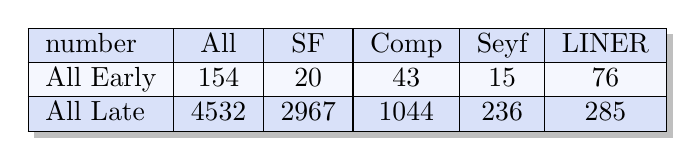
\begin{tikzpicture}
  \node[drop shadow,fill=white,inner sep=0pt] 
  {\rowcolors{1}{RoyalBlue!20}{RoyalBlue!5}
  \begin{tabular}{|l | c | c | c | c | c |}
  \hline
  number & All & SF & Comp & Seyf & LINER \\
  \hline
  All Early & 154 & 20 & 43 & 15 & 76  \\ 
  \hline
  All Late & 4532 & 2967 & 1044 & 236 & 285  \\
  \hline
  \end{tabular}
  };
  \end{tikzpicture}
  \end{center}
  \begin{center}
  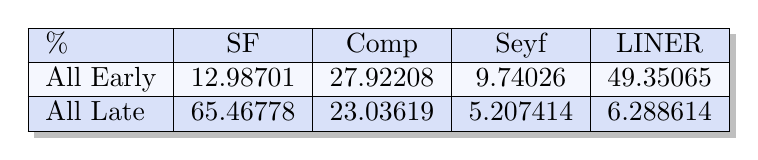
\begin{tikzpicture}
  \node[drop shadow,fill=white,inner sep=0pt] 
  {\rowcolors{1}{RoyalBlue!20}{RoyalBlue!5}
  \begin{tabular}{|l | c | c | c | c | }
  \hline
  \% & SF & Comp & Seyf & LINER \\
  \hline
  All Early& 12.98701 & 27.92208 & 9.74026 & 49.35065 \\ 
  \hline
  All Late & 65.46778 & 23.03619 & 5.207414 & 6.288614 \\
  \hline
  \end{tabular}
  };
  \end{tikzpicture}
  \end{center}
  
  \begin{itemize}
   \item  OSSY 제공 데이터의 관측 범위 내에서 Early type galaxy가 Late type galaxy보다 훨씬 적은 수의 표본을 가짐.
   따라서 단순 갯수 비교가 아닌 비율을 구해 봄.
   \item  Early type에선 LINER, Late type에선 SF의 비율이 높게 나타나는 것을 확인.
   \item  Seyfert galaxy중 Late type의 비율이 높지만, Early type중의 Seyfert galaxy의 비율이 Late type에서의 Seyfert galaxy비율보다 높았다.
  \end{itemize}
\end{frame}

\begin{frame}
 \frametitle{Emission Line}
 \SM
  \begin{columns}[t]
  \column{.55\textwidth}
   \begin{figure}
    \centering
    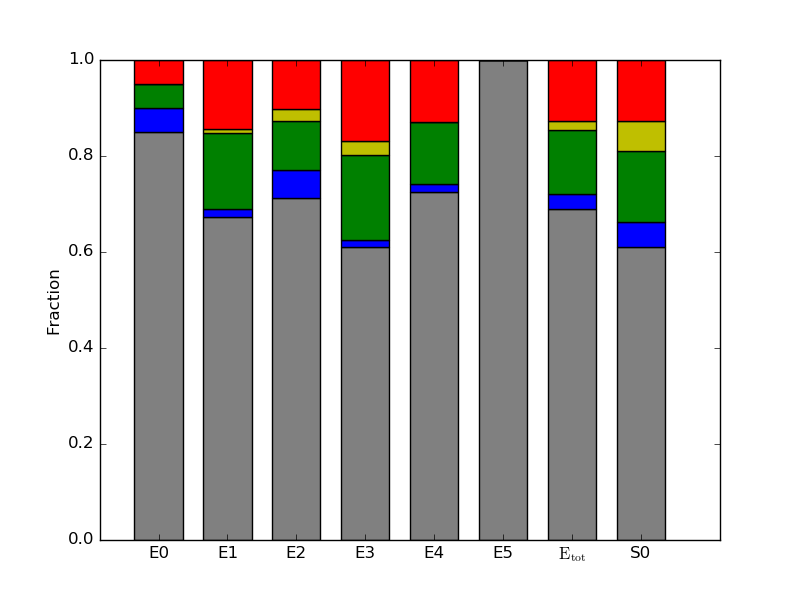
\includegraphics[width=6cm, height=4cm]{Earlybar.png}
   \end{figure}
   \column{.55\textwidth}
   \begin{figure}
    \centering
    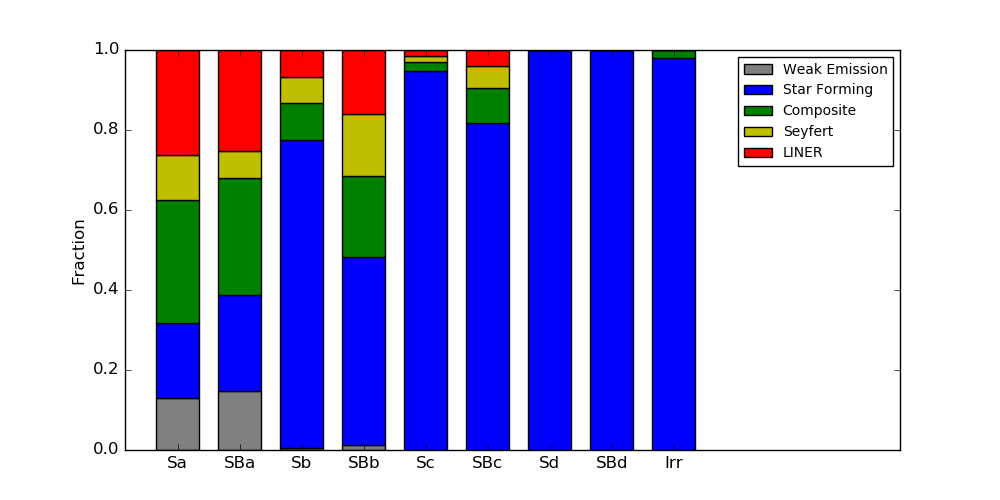
\includegraphics[width=6cm, height=4cm]{Latebar.png}
   \end{figure}
  \end{columns}
\vspace{0.2cm}
\begin{itemize}
 \item  Early type galaxy들은 galaxy morphology에 관계없이 Weak Emission line galaxy가 dominant하고 그 외에 LINER와 Composite계열의
 fraction이 높은 것을 확인할 수 있음.
 \item  Late type galaxy들은 이와 다르게, Sa(SBa)에서 Sd(SBd)로 갈수록 Star forming galaxy의 비중이 높아지는 것을 확인할 수 있음.
\end{itemize}
\end{frame}

\section{Radio Cross Match \& Radio Luminosity}

\begin{frame}
  \frametitle{BPT Diagram}
  \SM
  \begin{columns}
  \column{.65\textwidth}
   \begin{figure}
    \centering
    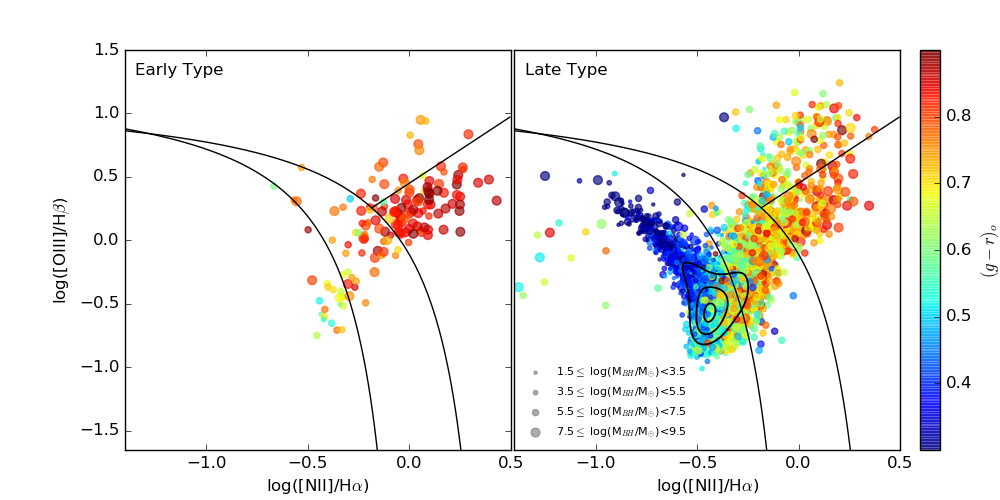
\includegraphics[width=7cm, height=4cm]{BPT.png}
   \end{figure}
   \column{.45\textwidth}
   \centering
   \begin{block}{BPT Diagram}
    \begin{itemize}
     \item 전체 : 4686개
     \begin{itemize}
      \item Early type : 154
      \item Late type : 4532
     \end{itemize}
    \end{itemize}
   \end{block}
  \end{columns}
  \vspace{0.2cm}
  앞에서 BPT diagram으로 각 은하의 Star formation과 AGN, Seyferts, LINERs에 대해 논의해 보았고, 이번에는 Radio wave에 대해
  관측되는 은하(Radio-active galaxies)와, 그렇지 않은 은하(Non-radio-active galaxies)에 대해 확인해 보도록 한다.
\end{frame}

\begin{frame}
  \frametitle{BPT Diagram of non-radio-active}
  \SM
  \begin{columns}
  \column{.65\textwidth}
   \begin{figure}
    \centering
    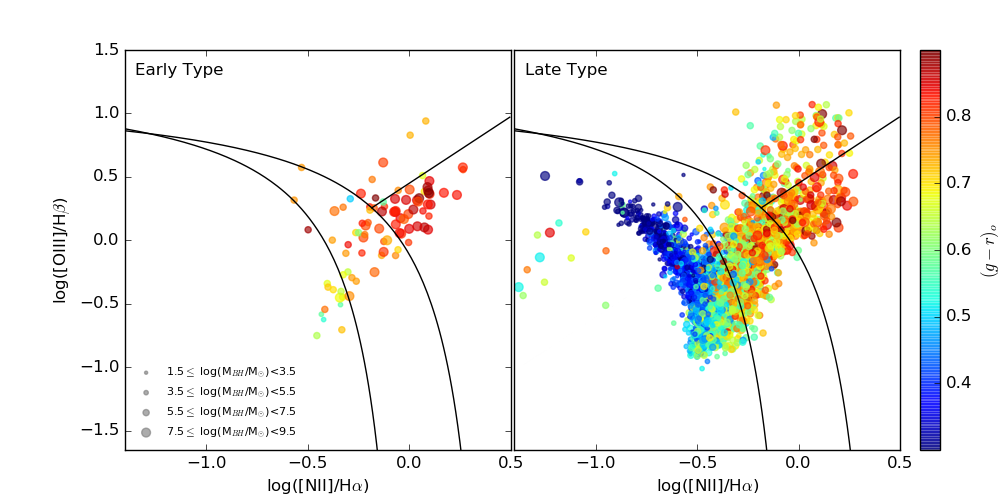
\includegraphics[width=7cm, height=3.5cm]{BPT_nonradio.png}
   \end{figure}
   \column{.45\textwidth}
   \centering
   \begin{block}{BPT Diagram}
    \begin{itemize}
     \item 전체 : 3893개
     \begin{itemize}
      \item Early type : 91
      \item Late type : 3802
     \end{itemize}
    \end{itemize}
   \end{block}
  \end{columns}
  \vspace{0.2cm}
  \textbf{앞 페이지의 4686개의 은하로 plot한 그래프와 비교 :}
  \begin{itemize}
   \item 전체적으로 그래프가 왼쪽 아래로 치우친 것을 볼 수 있음.
   \begin{itemize}
   \SSM
   \setbeamertemplate{itemize items}[triangle]
    \item AGN 영역의 감소 – AGN에서 전파가 방출됨을 간접적으로 추론
   \end{itemize}
   \item Late type에서의 Star Formation 영역의 변화 없음.
   \begin{itemize}
   \SSM
   \setbeamertemplate{itemize items}[triangle]
    \item SF 영역 변화 없음 – SF 과정의 은하는 전파를 방출하지 않음 확인
   \end{itemize}
   \item 질량을 의미하는 점의 크기의 감소
   \begin{itemize}
   \SSM
   \setbeamertemplate{itemize items}[triangle]
    \item Radio active galaxies의 경우 Massive Black hole을 가지고 있음 확인
   \end{itemize}
  \end{itemize}
\end{frame}

\begin{frame}
  \frametitle{BPT Diagram of Radio-active}
  \SM
  \begin{columns}
  \column{.65\textwidth}
   \begin{figure}
    \centering
    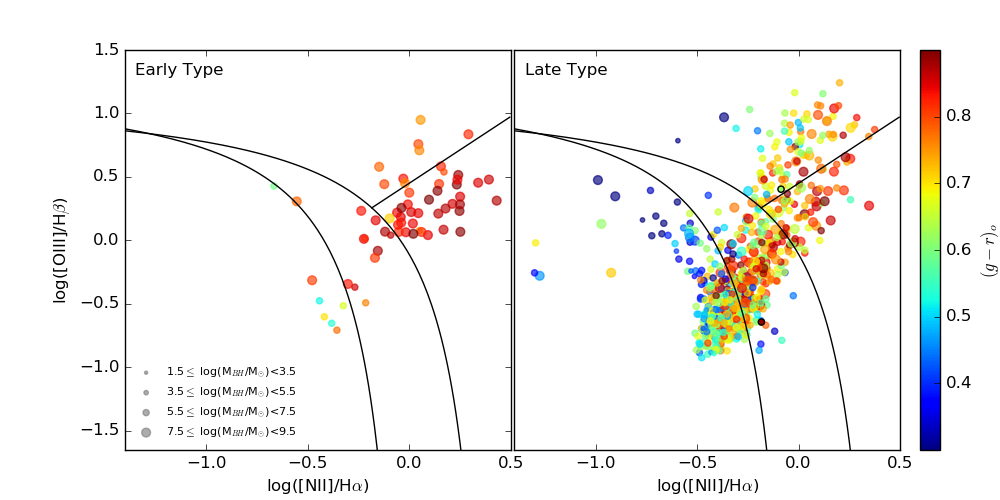
\includegraphics[width=7cm, height=3.5cm]{BPT_radio_Active.png}
   \end{figure}
   \column{.45\textwidth}
   \centering
   \begin{block}{BPT Diagram}
    \begin{itemize}
     \item 전체 : 793개
     \begin{itemize}
      \item Early type : 63
      \item Late type : 730
     \end{itemize}
    \end{itemize}
   \end{block}
  \end{columns}
  \vspace{0.2cm}
  \textbf{앞 페이지의 non-radio-active galaxies의 그래프와 비교 :}
  \begin{itemize}
   \item  Early type에서의 AGN 영역에 존재하는 은하 비율 증가.
   \begin{itemize}
   \SSM
   \setbeamertemplate{itemize items}[triangle]
    \item  AGN 영역 증가 – AGN에서 전파가 방출됨을 재확인
   \end{itemize}
   \item  Late type에서의 Star Formation 영역의 큰 감소
   \begin{itemize}
   \SSM
   \setbeamertemplate{itemize items}[triangle]
    \item  SF 영역의 감소 – SF 과정의 은하는 전파를 방출하지 않음 재확인
   \end{itemize}
  \end{itemize}
\end{frame}

\begin{frame}
  \frametitle{Classification - FR1: Centre Bright}
  \SM
  \begin{columns}
  \column{.55\textwidth}
   \begin{figure}
    \centering
    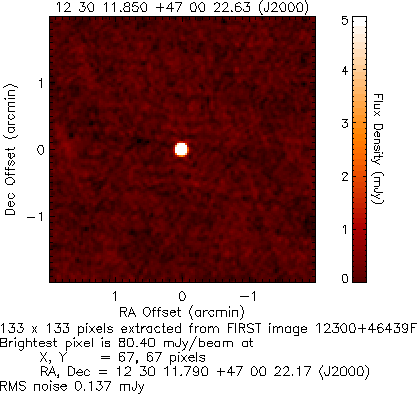
\includegraphics[width=5cm, height=3.5cm]{core.png}
   \end{figure}
   \column{.45\textwidth}
   \centering
   \begin{block}{Classification}
    \begin{itemize}
     \item 분류기준:
     
     Core의 밝기가 강해 Source가 하나로 보이는 은하를 기준으로 선정하였다.
     \vspace{0.2cm}
     \item 분류결과:
     
     이 결과 위에서 분류한 793개의 은하 중 786개의 은하를 FR1으로 분류하였다.
    \end{itemize}
   \end{block}
  \end{columns}
  \vspace{0.2cm}
 
\end{frame}

\begin{frame}
  \frametitle{Classification - FR2: Jet Bright}
  \SM
  \begin{columns}
  \column{.55\textwidth}
   \begin{figure}
    \centering
    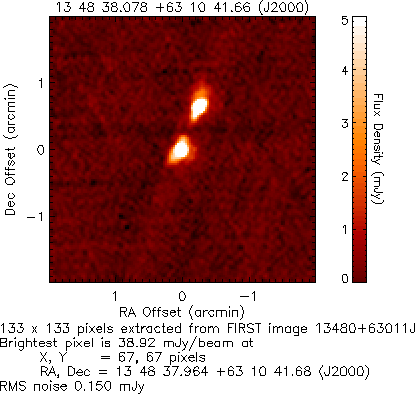
\includegraphics[width=5cm, height=3.5cm]{jet.png}
   \end{figure}
   \column{.45\textwidth}
   \centering
   \begin{block}{Classification}
    \begin{itemize}
     \item 분류기준:
     
     Core의 밝기보다 Jet의 밝기가 밝아, Source가 두 개로 보이는 은하를 기준으로 선정하였다.
     \vspace{0.2cm}
     \item 분류결과:
     
     이 결과 위에서 분류한 793개의 은하 중 7개의 은하를 FR2로 분류하였다.

    \end{itemize}
   \end{block}
  \end{columns}
  \vspace{0.2cm}
\end{frame}

\begin{frame}
  \frametitle{BPT Diagram of FR2}
  \SM
  \begin{columns}
  \column{.55\textwidth}
   \begin{figure}
    \centering
    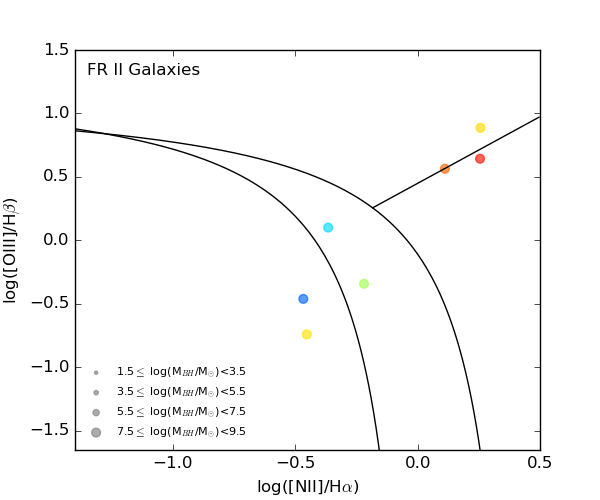
\includegraphics[width=4.5cm, height=3.5cm]{BPT_FR2.png}
   \end{figure}
   \column{.55\textwidth}
   \centering
   \begin{block}{BPT Diagram}
    \begin{itemize}
     \item 전체 : 793개
     \begin{itemize}
      \item FR1 Galaxies: 786
      \item \textbf{FR2 Galaxies : 7}
     \end{itemize}
    \end{itemize}
   \end{block}
  \end{columns}
  \vspace{0.2cm}
  FR2 galaxies의 BPT diagram에서, 7개 모두 Early type galaxy임을 확인.
Early type의 경우 Late type에 비해 core의 BH에 의한 물질의 소모 클 것임을
가정하면, 그 물질의 소모에 의한 감소가 core의 luminosity의 감소를 이끌었음
을 추론할 수 있다.
\end{frame}


\begin{frame}
 \frametitle{Correlation between Accretion rate \& Morphology}
 \SSM
  \begin{columns}
  \column{.55\textwidth}
   \begin{figure}
    \centering
    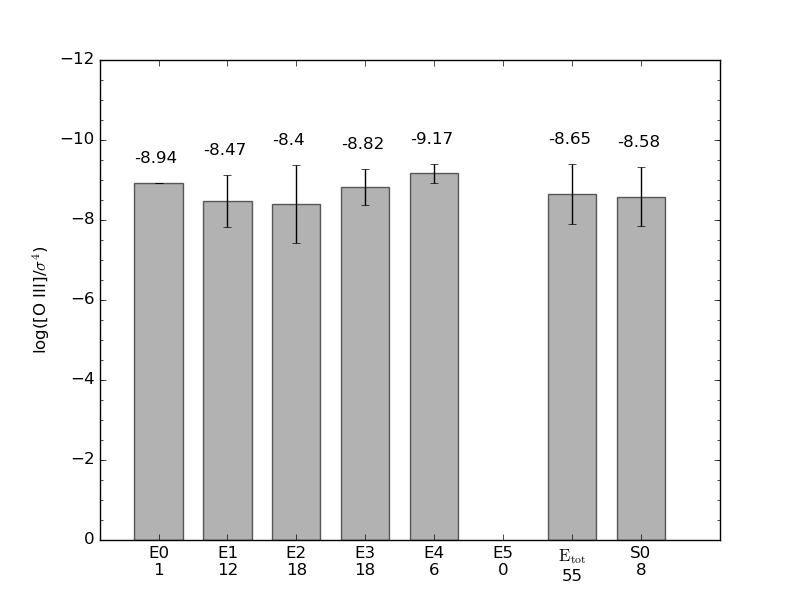
\includegraphics[width=5cm, height=2.5cm]{accearly.png}
    \hfill
    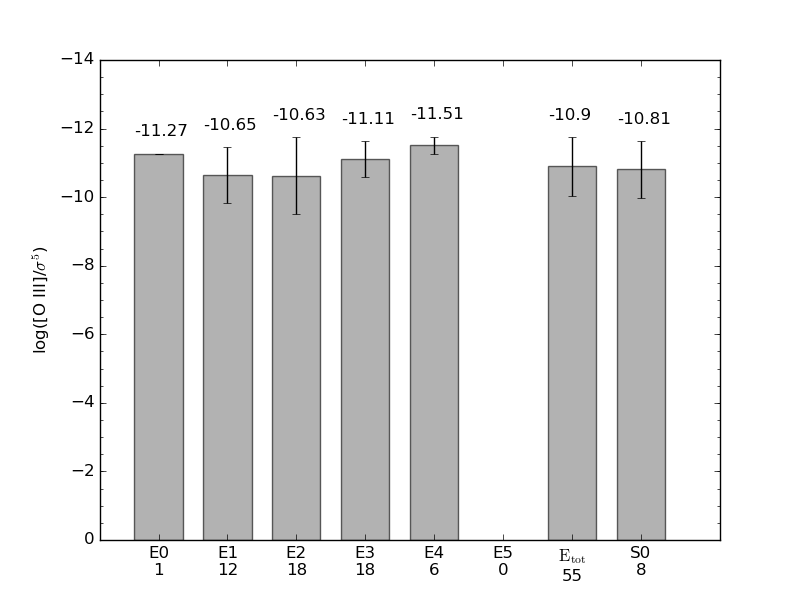
\includegraphics[width=5cm, height=2.5cm]{accearly2.png}
    \caption{Early type}
   \end{figure}
   \column{.55\textwidth}
   \begin{figure}
    \centering
    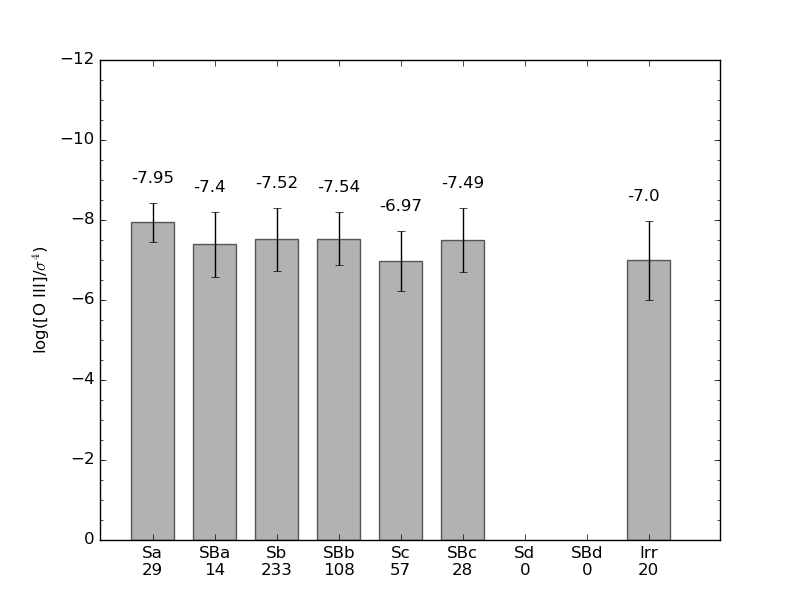
\includegraphics[width=5cm, height=2.5cm]{acclate.png}
    \hfill
    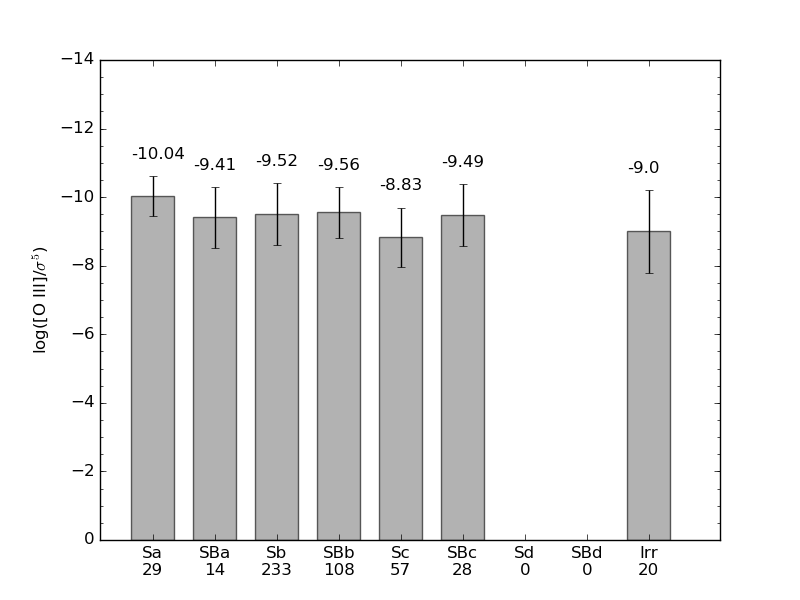
\includegraphics[width=5cm, height=2.5cm]{acclat2.png}
    \caption{Late type}
   \end{figure}
  \end{columns}
\vspace{0.2cm}
\end{frame}

\begin{frame}
 \frametitle{Correlation between Accretion rate \& Morphology}
 \SM
 \begin{block}{Comments}
  \begin{enumerate}
   \item Late type은 Early type에 비해 Emission line luminosity가 강함
   \vspace{0.2cm}
   
   $\therefore$ Center Black hole에서 가스를 소모하며 방출선을 내는데 Late type의 경우, 
   Early type에 비해 가스가 풍부하여 Emission line luminosity가 강함
   
   \item Sa type $\rightarrow$ Sc type 으로 갈 수록 [O3] line이 강해짐
   \vspace{0.2cm}
   
   $\therefore$ 분석 1의 결과를 바탕으로 Sc $\rightarrow$ Sa 방향으로 가스가 적어지므로, 분석 2의 결과를 예상할 수 있음
  \end{enumerate}
 \end{block}
\end{frame}

\begin{frame}
  \frametitle{Radio luminosity correlation}
  \SM
  \begin{columns}
  \column{.55\textwidth}
   \begin{figure}
    \centering
    \includegraphics[width=6cm, height=3.5cm]{radiolum.png}
   \end{figure}
   \column{.45\textwidth}
   \centering
   \begin{block}{Analyze}
    \begin{itemize}
     \item 분석1:
     
     Early type의 경우 Late type에 비해 BH의 질량이 크게 관측됨

     \vspace{0.2cm}
     \item 분석2:
     
     Early type의 경우 Late type에 비해 accretion rate가 작게 관측됨
    \end{itemize}
   \end{block}
  \end{columns}
  \vspace{0.2cm}
  \begin{itemize}
   \item 분석3:
   
   Early type의 경우 BH의 질량과 Radio luminosity 사이에 상관관계가 없음
   
   \item 분석4:
   
   Early type의 경우 accretion rate와 Radio luminosity 사이에 상관관계가 없음
  \end{itemize}
\end{frame}

\begin{frame}
 \frametitle{Radio luminosity correlation}
 \NM
 여기서 중점적으로 고려해봐야 하는 것은 분석 3, 4 이므로, 다음그림을 보자.
  \begin{columns}
  \column{.55\textwidth}
   \begin{figure}
    \centering
    \includegraphics[width=5cm, height=3.5cm]{acceffi.png}
   \end{figure}
   \column{.55\textwidth}
   \begin{figure}
    \centering
    \includegraphics[width=5cm, height=3.5cm]{cor.png}
   \end{figure}
  \end{columns}
  \vspace{0.2cm}
$\therefore$ BH의 질량과 accretion rate 사이에는 상관관계가 없음
\end{frame}


\end{document}
